%% Document class
%\documentclass[12pt,preprint]{aastex}
%\documentclass[preprint2]{aastex}
\documentclass[iop,revtex4]{emulateapj}

%general packages
\usepackage{amsmath}	%for \text{} in math mode
\usepackage{mathrsfs } %for likelihood L
\usepackage{lscape} % landscape environment

%%Figure packages
\usepackage{grffile}	%for dots in filenames
\usepackage{subfigure}

%%Referencinb
\usepackage{hyperref}

%% Custom macros
\newcommand{\vect}[1]{\boldsymbol{#1}} % Uncomment for BOLD vectors.
%\newcommand{\vect}[1]{\vec{#1}} % Uncomment for ARROW vectors.
\newcommand*\diff{\mathop{}\!\mathrm{d}}
\newcommand*\Diff[1]{\mathop{}\!\mathrm{d^#1}}
\newcommand{\pdf}{\ensuremath{pdf}}
\newcommand{\pmodel}{\ensuremath{p_M}}
\newcommand{\MAP}{MAP}
\newcommand{\MAPs}{MAPs}
\newcommand{\RM}{{\sl RoadMapping}}
\makeatletter
\newcommand{\testlabel}[2]{%
   \protected@write \@auxout {}{\string \newlabel {#1}{{#2}{\thepage}{#2}{#1}{}} }%
   \hypertarget{#1}{#2}
}
\makeatother
\usepackage[usenames,dvipsnames]{xcolor}
\newcommand{\Wilma}[1]{\textcolor{Fuchsia}{#1}}
\newcommand{\HW}[1]{\textcolor{Green}{#1}}
\newcommand{\Jo}[1]{\textcolor{Blue}{#1}}

%% Abbreviations
\shorttitle{Action-based Dynamical Models for the Milky Way}
\shortauthors{Trick et al.}

\begin{document}
 
%% Title [TO DO: Decide on one of them]
%\title{The {\sc RoadMapping} Code:\\How to deal with ``Real World'' Issues\\in Action-based Dynamical Modelling the Milky Way\\}
\title{Action-based Dynamical Modelling of the Milky Way Disk\\with \emph{RoadMapping}\\and our Imperfect Knowledge of the ``Real World''\\}

%% Authors    
\author{Wilma H. Trick\altaffilmark{1,2},  Jo Bovy\altaffilmark{3}, and Hans-Walter Rix\altaffilmark{1}}
%\email{trick@mpia.de}

%% Affiliations
\altaffiltext{1}{Max-Planck-Institut f\"ur Astronomie, K\"onigstuhl 17, D-69117 Heidelberg, Germany}
\altaffiltext{2}{Correspondence should be addressed to trick@mpia.de.}
\altaffiltext{3}{University of Toronto \Jo{[TO DO: What is Jo's current address???]}}


%-----------------------------------------------------------------------------------------------------------------------------------------------------------------------------
% Abstract
\begin{abstract}
We present \RM{}, a full-likelihood dynamical modelling machinery that aims to recover the Milky Way's (MW) gravitational potential from stellar sub-populations in the Galactic disk. \RM{} models the observed positions and velocities of stars with an equilibrium, three-integral distribution function (DF) in an axisymmetric potential and accounts also for survey selection effects. In preparation for the application to the large data sets of modern surveys like Gaia, we create and analyze a large suite of mock data sets and develop qualitative ``rules of thumb'' for which characteristics and limitations of data, model and machinery affect constraints on the potential and DF most. Overall we find that the potential can be reliably recovered if the model assumptions are fulfilled---and even if they are slightly wrong. 
\RM{} gives constraints of high precision for i) large sample sizes, ii) survey volumes of large radial and vertical coverage, iii) as long as the measurement uncertainties are perfectly known (even for proper motion uncertainties $\delta \mu \sim 5~\text{mas yr}^{-1}$). Unbiased estimates are ensured, for i) small to moderate misjudgements of the spatial selection function, ii) if distances are known to within $10\%$ (at least for distances smaller $3~\text{kpc}$), iii) if proper motion uncertainties are known within $10\%$ (at least for $\delta \mu \simeq 3~\text{mas yr}^{-1}$). Minor differences between the true and assumed DF are acceptable. When defining sub-populations by binning stars according to their chemical abundances, finite bin sizes and abundance errors would not affect the modelling as long as the DF parameters of neighbouring bins do not vary more than $20\%$. While hotter populations are less affected by pollution and misjudgements of $\delta \mu$, cooler populations recover the Galaxy rotation curve more reliably. If the Galaxy's true gravitational potential is not included in the assumed family of parametrized model potentials, we can---at least in the axisymmetric case---still find a potential that is a reliable fit within the limitations of the model. Challenges of the future are the rapidly increasing computational costs for high precision likelihood evaluations required for large sample sizes.
\end{abstract}






%-----------------------------------------------------------------------------------------------------------------------------------------------------------------------------

%% Keywords
\keywords{Galaxy: disk --- Galaxy: fundamental parameters --- Galaxy: kinematics and dynamics --- Galaxy: structure}

%-----------------------------------------------------------------------------------------------------------------------------------------------------------------------------
%Introduction
%\section{Introduction} \label{sec:intro}

%Everything in a nutshell
Stellar dynamical modelling can be employed to infer the Milky Way's (MW) gravitational potential from the positions and motions of individual stars (\citealt{2008gady.book.....B,2011Prama..77...39B,2013A&ARv..21...61R}). Observational information on the 6D phase-space coordinates of stars is currently growing at a rapid pace, and will be taken to a whole new level in number and precision by the upcoming data from the Gaia mission \citep{2001A&A...369..339P}. Yet, rigorous and practical modelling tools that turn position-velocity data of individual stars into constraints both on the gravitational potential and on the distribution function (DF) of stellar orbits, are scarce \citep{2013A&ARv..21...61R}.

%Why potential + DF are important
The Galactic gravitational potential is fundamental for understanding the MW's dark matter and baryonic structure \citep{2013A&ARv..21...61R,2012EPJWC..1910002M,2013PhR...531....1S,2014JPhG...41f3101R} and the stellar-population dependent orbit distribution function is a basic constraint on the Galaxy's formation history \citep{2013NewAR..57...29B,2013A&ARv..21...61R,2015MNRAS.449.3479S}.

%Action-based DF modelling in general
There is a variety of practical approaches to dynamical modelling of discrete collisionless tracers, such as the stars in the MW, e.g., Jeans modelling (\citealt{1989MNRAS.239..605K}, \citealt{2012ApJ...756...89B}, \citealt{2012MNRAS.425.1445G}, \citealt{2013ApJ...772..108Z}, \citealt{2015MNRAS.452..956B}), action-based DF modelling (\citealt{2013ApJ...779..115B}, \citealt{2014MNRAS.445.3133P}, \citealt{2015MNRAS.449.3479S}), torus modelling (\citealt{2008MNRAS.390..429M}, \citealt{2012MNRAS.419.2251M}, \citealt{2013MNRAS.433.1411M}), Made-to-measure modelling (\citealt{sye96}, \citealt{2007MNRAS.376...71D} or \citealt{2014MNRAS.443.2112H}). Most of them---explicitly or implicitly---describe the stellar distribution through a distribution function. 

%The roots of our approach
Recently, \citet{2012MNRAS.426.1328B} and \citet{2013ApJ...779..115B} \HW{[TO DO: are these the correct references???]} proposed to constrain the MWs gravitational potential by combining parametrized axisymmetric potentials models with DFs that are simple analytic functions of the three orbital actions (\citealt{2008gady.book.....B}, \S 3.5 \& \S 4.6, \citealt{2011Prama..77...39B}) to model discrete data.



%The first version of the code + first results
\citet{2013ApJ...779..115B} (BR13 hereafter) put this in practice by implementing a rigorous modelling approach for so-called mono-abundance populations (\MAPs{}), i.e, sub-sets of stars with similar $[\mathrm{Fe}/\mathrm{H}]$ and $[\alpha/\mathrm{Fe}]$ within the Galactic disk, which seem to allow simple DFs \citep{bov12b,bov12c,2012ApJ...753..148B}. Given an assumed axisymmetric model for the Galaxy potential and action-based DF \citep{2010MNRAS.401.2318B,2011MNRAS.413.1889B,2013MNRAS.434..652T} they calculated the likelihood of the observed ($\vec{x},\vec{v}$) for each \MAP{} among SEGUE G-dwarf stars \citep{2009AJ....137.4377Y}. They also accounted for the complex, but known selection function \citep{2012ApJ...753..148B} of the kinematic tracers. For each \MAP{} the modelling resulted in an independent estimate on the same gravitational potential. Taken as an ensemble, they constrained the disk surface mass density over a wide range of radii ($\sim 4-9$ kpc), and proved to be a powerful constraint on the disk mass scale length and on the disk-to-dark-matter ratio at the Solar radius. 

%Drawbacks of the first code version in the era of large surveys
BR13 made however a number of quite severe and idealizing assumptions about potential, DF and the knowledge of observational effects. These idealizations are likely to translate into systematic errors on the inferred potential, well above the formal error bars of the upcoming surveys with their wealth and quality of data.

%Focus of this work: Not just follow-up of BR13, but presentation and investigation of much improved machinery
In this work we present \RM{} (``\textsc{R}ecovery of the \textsc{O}rbit \textsc{A}ction \textsc{D}istribution of \textsc{M}ono-\textsc{A}bundance \textsc{P}opulations and \textsc{P}otential \textsc{IN}ference for our \textsc{G}alaxy'') - an improved, refined, flexible, robust and well-tested version of the original dynamical modelling machinery by BR13, explicitly developed to deal with large data sets. Our goal is to explore which of the assumptions BR13 made and which other aspects of data, model and machinery limit \RM{}'s recovery of the true gravitational potential.

%Large Data + Machinery
We investigate the following aspects of the \RM{} machinery that become especially important for a huge number of stars: (i) We have to make sure that \RM{} is an unbiased estimator (Section \ref{sec:largedata}). (ii) Numerical inaccuracies must not be an important source of systematics (Section \ref{sec:likelihood}). (iii) As parameter estimates become much more precise (Section \ref{sec:largedata}, we need more flexibility in the potential and DF model and effective strategies to find the best fit parameters. The improvements made in \RM{} as compared to the machinery used in BR13 are presented in Section \ref{sec:fitting}.

%Data 
We also explore how different aspects of the observational experiment design impact the parameter recovery: (i) It might be worth to explore the importance of the survey volume geometry, size, shape and position within the MW to constrain the potential (Section \ref{sec:results_obsvolume}). (ii) What if our knowledge of the sample selection function is imperfect, and potentially biased (Section \ref{sec:results_incompR})? (iii) How to best account for individual and possibly misjudged measurement uncertainties (Section \ref{sec:results_errors})? (iv) Given several stellar populations of different kinematic temperature---what is the best choice (Section \ref{sec:results_temperature})? 

%Model
One of the strongest assumptions is to restrict the dynamical modelling to a certain family of parametrized models. We investigate how well we can we hope to recover the true potential, when our models do not encompass the true DF (Section \ref{sec:results_mixedDFs}) and potential (Section \ref{sec:results_potential})

The most severe idealization that goes into this kind of dynamical modelling might be that of the Galaxy being axi-symmetric and in steady state. We do not investigate this within the scope of this paper but strongly suggest a systematic investigation of this for future work.

For all of the above aspects we show some plausible and illustrative examples on the basis of investigating mock data. The mock data is generated from galaxy models presented in Sections \ref{sec:coordinates}-\ref{sec:selectionfunction} following the procedure in Section \ref{sec:mockdata}, analysed according to the description of the \RM{} machinery in Sections \ref{sec:likelihood}-\ref{sec:fitting} and the results are presented in Section \ref{sec:results} and discussed in Section \ref{sec:discussionsummary}.

\HW{[TO DO: Jo wanted more details on tests in introduction. Any ideas what exactly?]}

%-----------------------------------------------------------------------------------------------------------------------------------------------------------------------------

%-----------------------------------------------------------------------------------------------------------------------------------------------------------------------------
%Dynamical Modelling
\section{Dynamical Modelling}


%=============================================

\begin{deluxetable*}{lllrl}
\tabletypesize{\scriptsize}
\tablecaption{Gravitational potentials of the reference galaxies used troughout this work and the respective ways to calculate actions in these potentials. All four potentials are axisymmetric. The potential parameters are fixed for the mock data creation at the values given in this table. In the subsequent analyses we aim to recover these potential parameters again. The parameters of \texttt{MW13-Pot} and \texttt{KKS-Pot} were chosen to resemble the \texttt{MW14-Pot} (see Figure \ref{fig:ref_pots}). We use $v_\text{circ}(R_\odot)$ = $230$ km s$^{-1}$ for all potentials in this work. \label{tbl:referencepotentials}}
\tablewidth{0pt}
\tablehead{
\colhead{name} & \colhead{potential type} & \multicolumn{2}{c}{potential parameters $p_\Phi$} & \colhead{action calculation}}
\startdata
\texttt{Iso-Pot}      & isochrone potential\tablenotemark{(a)} & $b$& $0.9~\text{kpc}$ & \textbf{\emph{analytical and exact}} \\
                               & \citep{1959AnAp...22..126H} &                                            &                               & (\citealt{2008gady.book.....B}, \S 3.5.2) \\
\tableline
\texttt{KKS-Pot}    & 2-component                            & $\Delta$                                              & $0.3$   & \textbf{\emph{exact}} \\
                               & Kuzmin-Kutuzov-                      & $\left(\frac{a}{c}\right)_\text{Disk}$ & $20$    & using \emph{St\"{a}ckel Fudge} \\ 
                               & St\"{a}ckel potential\tablenotemark{(b)} & $\left(\frac{a}{c}\right)_\text{Halo}$ & $1.07$ & \citep{2012MNRAS.426.1324B} \\
                               & \hspace{0.3cm} (disk + halo) & $k$                                                       & $0.28$ & and interpolation \\
                               & \citep{1994AA...287...43B}                               &                                                              &               & on action grid\tablenotemark{(e)} \\
                               &                                                       &                                                              &                & \citep{2015ApJS..216...29B} \\
\tableline
\texttt{MW13-Pot} & MW-like potential\tablenotemark{(c)} with & $R_d$ & $3~\text{kpc}$ & \textbf{\emph{approximate}} \\ 
                               & Hernquist bulge,                         & $z_h$ & $0.4~\text{kpc}$  & (same as \texttt{KKS-Pot}) \\
                               & spherical power-law halo,        & $f_h$ & $0.5$ & \\
                               & 2 exponential disks                    & $\frac{\diff \ln(v_\text{circ}(R_\odot))}{ \diff \ln(R)}$ & $0$  & \\
                               & \hspace{0.3cm} (stars + gas)  &  & & \\
                               & \citep{2013ApJ...779..115B} & & &\\
\tableline
\texttt{MW14-Pot} & MW-like potential\tablenotemark{(d)} with &  & & \textbf{\emph{approximate}} \\
                               & cut-off power-law bulge, & & & (same as \texttt{KKS-Pot}) \\
                               & Miyamoto-Nagai stellar disk, & & & \\
                               & NFW halo & & & \\
                               & \citep{2015ApJS..216...29B} & & & \\
\enddata
\tablenotetext{(a)}{The isochrone potential \texttt{Iso-Pot} has one free parameter, the scale length $b$.} 
\tablenotetext{(b)}{The coordinate system of each of the two St\"{a}ckel-potential components of the \texttt{KKS-Pot} is $\frac{R^2}{\tau_{i,p}+\alpha_p} + \frac{z^2}{\tau_{i,p}+\gamma_p}=1$ with $p \in \{\text{Disk},\text{/Halo}\}$ and $\tau_{i,p} \in \{\lambda_p,\nu_p\}$. Both components have the same focal distance $\Delta \equiv \sqrt{\gamma_p-\alpha_p}$, to make sure that the superposition of the two components itself is still a St\"{a}ckel potential. The axis ratio of the coordinate surfaces $\left(\frac{a}{c}\right)_p := \sqrt{\frac{\alpha_p}{\gamma_p}}$ describes the flatness of the corresponding St\"{a}ckel component. The parameter $k$ describes the relative contribution of the disk mass to the total mass.} 
\tablenotetext{(c)}{The free parameters of the \texttt{MW13-Pot} are stellar disk scale length $R_d$ and height $z_d$, as well as the relative halo contribution to $v_\text{circ}^2(R_\odot)$, $f_h$, and the slope of the rotation curve, $\frac{\diff \ln(v_\text{circ}(R_\odot))}{ \diff \ln(R)}$.} 
\tablenotetext{(d)}{The \texttt{MWPotential2014} by \citet{2015ApJS..216...29B} (see their Table 1) has a circular velocity at the Sun of $v_\text{circ}(R_\odot)$ = $220$ km s$^{-1}$. In this work we use however $v_\text{circ}(R_\odot)$ = $230$ km s$^{-1}$ for all potentials.} 
\tablenotetext{(e)}{We use a finely spaced action interpolation grid with $R_\text{max}=10$ \Jo{[TO DO: What's that??? units???]} and 50 grid points in $E$ and $\psi$ \Jo{[TO DO: Find out what's that???]}, and 60 grid points in $L_z$.}
\end{deluxetable*}


%=============================================

\begin{deluxetable*}{lccccc}
\tabletypesize{\scriptsize}
\tablecaption{Reference distribution-function parameters for the qDF in Equations (\ref{eq:df_general})-(\ref{eq:sigmazRg}). These qDFs describe the phase-space distribution of stellar \MAPs{} for which mock data is created and analysed throughout this work for testing purposes. The parameters of the \texttt{cooler} \& \texttt{colder}  (\texttt{hotter} \& \texttt{warmer}) \MAPs{} were chosen to have the same $\sigma_{R,0}/\sigma_{z,0}$ ratio as the \texttt{hot} (\texttt{cool}) \MAP{}. The \texttt{colder} and \texttt{warmer} \MAPs{} have a free parameter $X$ that governs how much colder/warmer they are then the reference \texttt{hot} and \texttt{cool} qDFs. Hotter populations have shorter tracer scale lengths \citep{2012ApJ...753..148B} and the velocity dispersion scale lengths were fixed according to \citet{bov12c}. \label{tbl:referenceMAPs}}
\tablewidth{0pt}
\tablehead{
\colhead{name} & \multicolumn{5}{c}{qDF parameters $p_\text{DF}$}\\
                       & \colhead{$h_R$ [kpc]} & \colhead{$\sigma_{R,0}$ [km s$^{-1}$]} & \colhead{$\sigma_{z,0}$ [km s$^{-1}$]} & \colhead{$h_{\sigma,R}$ [kpc]} & \colhead{$h_{\sigma,z}$ [kpc]}}
\startdata
\texttt{hot}    & 2   & 55 & 66 & 8 & 7\\
\texttt{cool}   & 3.5 & 42 & 32 & 8 & 7\\
\tableline
\texttt{cooler} & 2  +50\% & 55-50\% & 66-50\% & 8 & 7 \\
\texttt{hotter} & 3.5-50\% & 42+50\% & 32+50\% & 8 & 7\\
\tableline
\texttt{colder} & 2  +X\% & 55-X\% & 66-X\% & 8 & 7 \\
\texttt{warmer} & 3.5-X\% & 42+X\% & 32+X\% & 8 & 7\\
\enddata
\end{deluxetable*}

%=============================================

%============================================



\Wilma{[TO DO: HW: In this section you have to indicate somehow, where you recapitulate BR13 and what is added new. "as in BR13", "beyond BR13"]}
\Wilma{TO DO: Comment from Hans-Walter: Basics of the method (binney, BR13) can be dramatically shortened. No need to sing the praises of \\DF's and actions. }

In this section we summarize the basic elements of \RM{}, the dynamical modelling machinery presented in this work, which in many respects follows \citet{2013ApJ...779..115B}.

\subsection{Coordinate System} \label{sec:coordinates}

Our modelling takes place in the Galactocentric rest-frame with cylindrical coordinates $\vect{x} \equiv (R,\phi,z)$ and corresponding velocity components $\vect{v} \equiv (v_R,v_\phi,v_z)$. If the stellar phase-space data is given in observed heliocentric coordinates, position $\tilde{\vect{x}} \equiv(\text{RA},\text{DEC},m-M)$ in right ascension RA, declination DEC and distance modulus $(m-M)$ as proxy for the distance from the sun, and velocity $\tilde{\vect{v}} \equiv (\mu_\text{RA},\mu_\text{DEC},v_\text{los})$ as proper motions $\vect{\mu}=(\mu_\text{RA},\mu_\text{DEC})$ \Jo{[TO DO: cos somwhere???]} in both RA and DEC direction and line-of-sight velocity $v_\text{los}$, the data $(\tilde{\vect{x}},\tilde{\vect{v}})$ has to be converted first into the Galactocentric rest-frame coordinates $(\vect{x},\vect{v})$ using the sun's position and velocity. We assume for the sun
\begin{eqnarray*}
(R_\odot,\phi_\odot,z_\odot) &=&(8 \text{ kpc}, 0^\circ, 0 \text{ kpc})\\
(v_{R,\odot},v_{T,\odot},v_{z,\odot}) &=& (0,230,0) \text{ km s}^{-1}.
\end{eqnarray*}

\subsection{Actions and Potential Models}  \label{sec:potentials}


Orbits in axisymmetric potentials are best described and fully specified by the three actions $\vect{J} \equiv (J_R, J_z, J_\phi=L_z)$, defined as
\begin{equation}
J_i = \frac{1}{2\pi} \oint_\text{orbit} p_i \diff x_i, \label{eq:action_general}
\end{equation}
and which depend on the potential via the connection between position $x_i$ and momentum $p_i$ along the orbit. Actions have a clear physical meaning: They quantify the amount of oscillation in each coordinate direction of the full orbit \HW{[TO DO: REF: HW suggested \citet{2008gady.book.....B}, but I can't find a corresponding statement in the book]}. The position of a star along the orbit is denoted by a set of angles, which form together with the angles a set of canonical conjugate phase-space coordinates (\citealt{2008gady.book.....B}, \S 3.5.1). \\

Even though actions are excellent orbit labels and arguments for stellar distribution functions, their computation is typically very expensive and depends on the choice of potential in which the star moves. The spherical isochrone potential \citep{1959AnAp...22..126H} is the only \Jo{[TO DO: Jo suggested "most general Galactic" instead of "only", but the isochrone is actually not Galactic... Ask him.]} potential for which Equation \ref{eq:action_general} takes an analytic form (\citealt{2008gady.book.....B}, \S 3.5.2). For St\"{a}ckel potentials actions can be calculated exactly by the (numerical) evaluation of a single integral. In all other potentials numerically calculated actions will always be approximations, unless Equation \ref{eq:action_general} is integrated along the whole (often not periodic) orbit.  A computational fast way to get actions for arbitrary axisymmetric potentials is the \emph{St\"{a}ckel fudge} by \citet{2012MNRAS.426.1324B}, which locally approximates the potential by a St\"{a}ckel potential. To speed up the calculation even more, an interpolation grid for $J_R$ and $J_z$ in energy $E$, angular momentum $L_z$ and \Jo{[TO DO: what else???]} can be build out of these St\"{a}ckel fudge actions, as described in \citet{2015ApJS..216...29B}.\\

For the gravitational potential in our modelling we assume a family of parametrized potential models with a fixed number of free parameters. We use different kinds of potentials: The Milky Way like potential from \citet{2013ApJ...779..115B} (\texttt{MW13-Pot}) with bulge, disk and halo; the spherical isochrone potential (\texttt{Iso-Pot}) in our test suites to make use of the analytic (and therefore exact and fast) way  to calculate actions; and the 2-component Kuzmin-Kutuzov St\"{a}ckel potential (\citealt{1994AA...287...43B}; \texttt{KKS-Pot}), which displays a disk and halo structure and also provides exact actions. Table \ref{tbl:referencepotentials} summarizes all reference potentials together used in this work with their free parameters $p_\Phi$. The density distribution of these potentials is illustrated in Figure \ref{fig:ref_pots}.\\

%=============================================

%FIGURE: reference potentials

\begin{figure*}[t]
\includegraphics[width=\textwidth]{figs/reference_potentials.eps}
\caption{Density distribution of the four reference galaxy potentials in Table \ref{tbl:referencepotentials}, for illustration purposes. These potentials are used throughout this work for mock data creation and potential recovery. \Wilma{[TO DO: Potential and/or population names in typewriter]}}
\label{fig:ref_pots}
\end{figure*}




%======================================================================================




\subsection{Stellar Distribution Functions} \label{sec:qDF}

Throughout, we assume that the orbits of each \MAP{} can be described by a single qDF of the form given by \citet{2011MNRAS.413.1889B}. This is motivated by the findings of \citet{bov12b,bov12c,2012ApJ...753..148B} and \citet{2013MNRAS.434..652T} about the simple phase-space structure of \MAPs{}, and following \citet{2013ApJ...779..115B} and their successful application. This qDF has the form
\begin{eqnarray}
&&\text{qDF}(\vect{J} \mid p_\text{DF}) \nonumber\\
&&= f_{\sigma_R}\left(J_R,L_z \mid p_\text{DF}\right) \times f_{\sigma_z}\left(J_z,L_z \mid p_\text{DF}\right)\label{eq:df_general}\end{eqnarray}
with
\begin{eqnarray}
f_{\sigma_R}\left(J_R,L_z \mid p_\text{DF}\right) &=& n \times \frac{\Omega}{\pi\sigma_R^2(R_g) \kappa}\exp\left(-\frac{\kappa J_R}{\sigma_R^2(R_g)} \right) \nonumber\\
&& \times \left[1+\tanh\left(L_z/L_0\right) \right]\\
f_{\sigma_z}\left(J_z,L_z \mid p_\text{DF} \right) &=& \frac{\nu}{2 \pi \sigma_z^2(R_g)} \exp\left( -\frac{\nu J_z}{\sigma_z^2(R_g)} \right).
\end{eqnarray}
Here $R_g \equiv R_g(L_z)$ and $\Omega\equiv \Omega(L_z)$ are the (guiding-center) radius and the circular frequency of the circular orbit with angular momentum $L_z$ in a given potential. $\kappa\equiv \kappa(L_z)$ and $\nu\equiv \nu(L_z)$ are the radial/epicycle ($\kappa$) and vertical ($\nu$) frequencies with which the star would oscillate around the circular orbit in $R$- and $z$-direction when slightly perturbed (\citealt{2008gady.book.....B}, \S 3.2.3) \Jo{[TO DO: ask someone, if I'm messing up different definitions of $\kappa$]}. The term $\left[1+\tanh\left(L_z/L_0\right) \right]$ suppresses counter-rotation for orbits in the disk with $L \gg L_0$ which we set to a small value ($L_0 = 10 \times R_\odot/8 \times v_\text{circ}(R_\odot)/220$ \Jo{[TO DO: Jo said, galpy default is 10 km/s kpc. But I got the value actually from the code...]}).
\\To match the observed properties of \MAPs{} (see \citealt{bov12b,bov12c,2012ApJ...753..148B}), we chose the functional forms
\begin{eqnarray}
n(R_g \mid p_\text{DF}) &\propto& \exp\left(-\frac{R_g}{h_R} \right)\\
\sigma_R(R_g \mid p_\text{DF}) &=& \sigma_{R,0} \times \exp\left(- \frac{R_g-R_\odot}{h_{\sigma,R}} \right)\label{eq:sigmaRRg}\\
\sigma_z(R_g \mid p_\text{DF}) &=& \sigma_{z,0} \times \exp\left(- \frac{R_g-R_\odot}{h_{\sigma,z}} \right)\label{eq:sigmazRg},
\end{eqnarray}
which indirectly set the stellar number density and radial and vertical velocity dispersion profiles. The qDF for each \MAP{} has therefore a set of five free parameters $p_\text{DF}$: the density scale length of the tracers $h_R$, the radial and vertical velocity dispersion at the solar position $R_\odot$, $\sigma_{R,0}$ and $\sigma_{z,0}$, and the scale lengths $h_{\sigma,R}$ and $h_{\sigma,z}$, that describe the radial decrease of the velocity dispersion. Throughout this work we use for illustration purposes a few example stellar populations, each following a single qDF, whose parameters are given in in Table \ref{tbl:referenceMAPs}. Most tests use the \texttt{hot} and \texttt{cool} qDFs from Table \ref{tbl:referenceMAPs}, which correspond to kinematically hot and cool populations, respectively.\\

One crucial point in our dynamical modelling technique (\S\ref{sec:likelihood}), as well as in creating mock data (\S\ref{sec:mockdata}), is to calculate the (axisymmetric) spatial tracer density $\rho_\text{DF}(\vect{x} \mid p_{\Phi},p_\text{DF})$ for a given qDF and potential . We do this by integrating the qDF at a given $(R,z)$ over all three velocity components, using a $N_v$-th order Gauss-Legendre quadrature for each integral:
\begin{eqnarray}
&&\rho_\text{DF}(R,|z| \mid p_{\Phi},p_\text{DF}) \nonumber\\
&&= \int_{-\infty}^{\infty} \text{qDF}(\vect{J}[R,z,\vect{v} \mid p_{\Phi}] \mid p_\text{DF}) \Diff3\vect{v}  \\%\label{eq:tracerdensity_general}\\
&&\approx \int_{-n_\sigma \sigma_R(R \mid p_\text{DF})}^{n_\sigma \sigma_R(R \mid p_\text{DF})} \int_{-n_\sigma\sigma_z(R \mid p_\text{DF})}^{n_\sigma \sigma_z(R \mid p_\text{DF})} \int_{0}^{1.5 v_\text{circ}(R_\odot)}  \nonumber\\
& & \hspace{1cm} \text{qDF}(J[R,z,\vect{v} \mid p_{\Phi}] \mid p_\text{DF}) \diff v_T \diff v_z \diff v_R, \label{eq:tracerdensity}
\end{eqnarray}
where $\sigma_R(R \mid p_\text{DF})$ and $\sigma_z(R \mid p_\text{DF})$ are given by Equations \ref{eq:sigmaRRg} and \ref{eq:sigmazRg} and the integration ranges are motivated by Figure \ref{fig:kks2WedgeEx}. The integration range $[0,1.5 v_\text{circ}(R_\odot)]$ over $v_T$ is in general sufficient (only for observation volumes at smaller Galactocentric radii with larger velocities this upper limit needs to be increased). For a given $p_\Phi$ and $p_\text{DF}$ we explicitly calculate the density on $N_x \times N_x$ regular grid points in the $(R,z)$ plane; in between grid points the density is evaluated with a bivariate spline interpolation. The grid is chosen to cover the extent of the observations (for $|z|\leq0$, because the model is symmetric in $z$ by construction). The total number of actions that need to be calculated to set up the density interpolation grid is $N_x^2 \cdot N_v^3$. \S\ref{sec:likelihood} and Figure \ref{fig:norm_accuracy} show the importance of choosing $N_x$, $N_v$ and $n_\sigma$ sufficiently large in order to get the density with an acceptable numerical accuracy \Wilma{[TO DO: Jo thinks that this statement is difficult to understand here, because you have not yet talked about the normalization]}. 


\subsection{Selection Functions} \label{sec:selectionfunction}

Any survey's selection function can be understood as defining an effective sample subvolume in the space of observables: e.g. position on the plane of the sky (the survey area), distance from the sun (limited by the brightness of the stars and the sensitivity of the detector), colors and metallicity of the stars (limited by survey mode and targeting).
\\We simply use spatial selection functions, which describe the probability to observe a star at $\vect{x}$,
\begin{eqnarray*}
\text{sf}(\vect{x}) \equiv \begin{cases}
\text{completeness}(\vect{x}) &\text{if $\vect{x}$ within observed volume}\\
0 & \text{outside.}
\end{cases}
\end{eqnarray*}
For the observed volume we use simple geometrical shapes. Either a sphere of radius $r_\text{max}$ with the sun at its center, or an angular segment of an cylindrical annulus (\texttt{wedge}), i.e. the volume with $R \in [R_\text{min},R_\text{max}],\phi \in [\phi_\text{min},\phi_\text{max}],z \in [z_\text{min},z_\text{max}]$ within the model galaxy. The sharp outer cut of the survey volume could be understood as the detection limit in apparent brightness in the case, where all stars have the same luminosity. Here $0 \leq \text{completeness}(\vect{x}) \leq 1$ everywhere inside the observed volume, so it can be understood as a position-dependent detection probability. Unless explicitly stated otherwise, we simplify to $\text{completeness}(\vect{x}) = 1$.

%%====================================================================

%FIGURE: accuracy in the likelihood normalisation 

\begin{figure*}[!htbp]
\centering
\plotone{figs/normalisation_accuracy_4.eps}
\caption{Relative error of the likelihood normalization, $\delta M_\text{tot}$, in Equation \ref{eq:relerrlikelihood} depending on the accuracy of the grid-based density calculation in Equation \ref{eq:tracerdensity} (and surrounding text) in five spherical observation volumes with different radius $r_\text{max}$. (Test \ref{test:norm_accuracy} in Table \ref{tbl:tests} summarizes the model parameters.) The tracer density in Equation \ref{eq:tracerdensity} is calculated on $N_x\times N_x$ spatial grid points in $R \in [R_\odot \pm r_\text{max}]$ and $|z| \in [0,r_\text{max}]$. The integration over the velocities is performed with Gauss-Legendre quadratures of order $N_v$ within an integration range of $\pm n_\sigma$ times the dispersion $\sigma_R(R)$ and $\sigma_z(R)$ (and $[0,1.5v_\text{circ}]$ in $v_T$). (We vary $N_x$, $N_v$ and $n_\sigma$ separately and keep the other two fixed at the values indicated above the columns.) We calculate the ``true'' normalization in Equation \ref{eq:relerrlikelihood} with high accuracy as $M_\text{tot} \equiv M_\text{tot,approx}(N_x=20,N_v=56,n_\sigma=7)$. The black dots indicate the accuracy used in our analyses: It is better than $0.001\%$ (dotted line). We find that the accuracy depends on the \emph{spatial} resolution of the grid and requires more accurate integrations over the \emph{velocity} for larger volumes within which the density varies more strongly.}
\label{fig:norm_accuracy}
\end{figure*}

%=============================================================


\subsection{Mock Data} \label{sec:mockdata}

We will rely on mock data as input to explore the limitations of the modelling. We assume that the positions and velocities of our stellar mock sample are indeed drawn from our assumed family of potentials and DFs (with given parameters $p_\Phi$ and $p_\text{DF}$). The DF is in terms of actions, while the transformation $(\vect{x}_i,\vect{v}_i) \longrightarrow \vect{J}_i$ is computationally much less expensive than the inversion. We therefore employ the following effective two-step method for creating mock data, which also accounts for a survey SF.

In the first step we draw stellar positions $\vect{x}_i$. We start by setting up the interpolation grid for the tracer density $\rho(R,|z| \mid p_\Phi, p_\text{DF})$ generated according to Section \ref{sec:qDF}.\footnote{For the creation of the mock data we use $N_x = 20$, $N_v = 40$ and $n_\sigma=5$ in Equation \ref{eq:tracerdensity}.} Next, we sample random positions $(R_i,z_i,\phi_i)$ uniformly within the observable volume. Using a Monte Carlo rejection method we then shape the sample to follow $\rho(R,|z| \mid p_\Phi, p_\text{DF})$. To apply a non-uniform SF$(\vect{x})$, we use the rejection method a second time. The resulting set of positions $\vect{x}_i$ follows the distribution$p(\vect{x}) \propto \rho_\text{DF}(R,|z| \mid p_{\Phi},p_\text{DF}) \times \text{SF}(\vect{x})$.

In the second step we draw velocities $\vect{v}_i$. For each of the positions $(R_i,z_i)$ we first sample velocities from a Gaussian envelope function in velocity space which is then shaped towards DF$(\vect{J}[R_i,z_i,\vect{v} \mid p_{\Phi}] \mid p_\text{DF})$ using a rejection method. We now have a mock data set satisfying $(\vect{x}_i,\vect{v}_i) \longrightarrow p(\vect{x},\vect{v}) \propto \text{DF}(\vect{J}[\vect{x},\vect{v} \mid p_{\Phi}] \mid p_\text{DF}) \times \text{SF}(\vect{x})$.

%====================================================================

Figure \ref{fig:kks2WedgeEx} shows examples of mock data sets in configuration space $(\vect{x},\vect{v})$ and action space. The mock data from the qDF lead to the expected distributions in configuration space. The distribution in action space illustrates the intuitive physical meaning of actions: The stars of the \texttt{cool} population have in general lower radial and vertical actions, as they are on more circular orbits. Circular orbits with $J_R = 0$ and $J_z = 0$ can only be observed in the Galactic mid-plane. The different ranges of angular momentum $L_z$ in the two example observation volumes reflect $L_z \sim R  \times v_\text{circ}$ and the volumes' different radial extent. The volume at larger $z$ contains stars with higher $J_z$.  An orbit with $L_z \ll$ or $\gg L_z(R_\odot)$ can only reach into a volume at $\sim R_\odot$, if it is more eccentric and has therefore larger $J_R$. This together with the effect of asymmetric drift explains the asymmetric distribution of $J_R$ vs. $L_z$ in Figure \ref{fig:kks2WedgeEx}.


Measurement uncertainties can be added to the mock data by applying the following modifications to the above procedure. We assume Gaussian uncertainties in the heliocentric phase-space coordinates $\tilde{\vect{x}} = (\text{RA},\text{Dec},(m-M)), \tilde{\vect{v}} = (\mu_\text{RA} \cdot \cos \text{Dec} ,\mu_\text{Dec},v_\text{los})$ (see Section \ref{sec:coordinates}), where we have taken $(m-M)$ as a proxy for distance. In the case of distance uncertainties $\delta(m-M)$, stars virtually scatter in and out of the observed volume. To account for this, we draw the \emph{true} $\vect{x}_i$ from a volume that is larger than the actual observation volume, perturb the $\vect{x}_i$ according to the position uncertainties and then reject all stars that lie now outside of the observed volume. This mirrors the Poisson scatter around the detection threshold for stars whose distances are determined from the apparent brightness and the distance modulus. We then sample \emph{true} $\vect{v}_i$ (given the \emph{true} $\vect{x}_i$) as described above and perturb them according to the velocity uncertainties.


%=============================================================


\begin{figure}[!htbp]
\centering
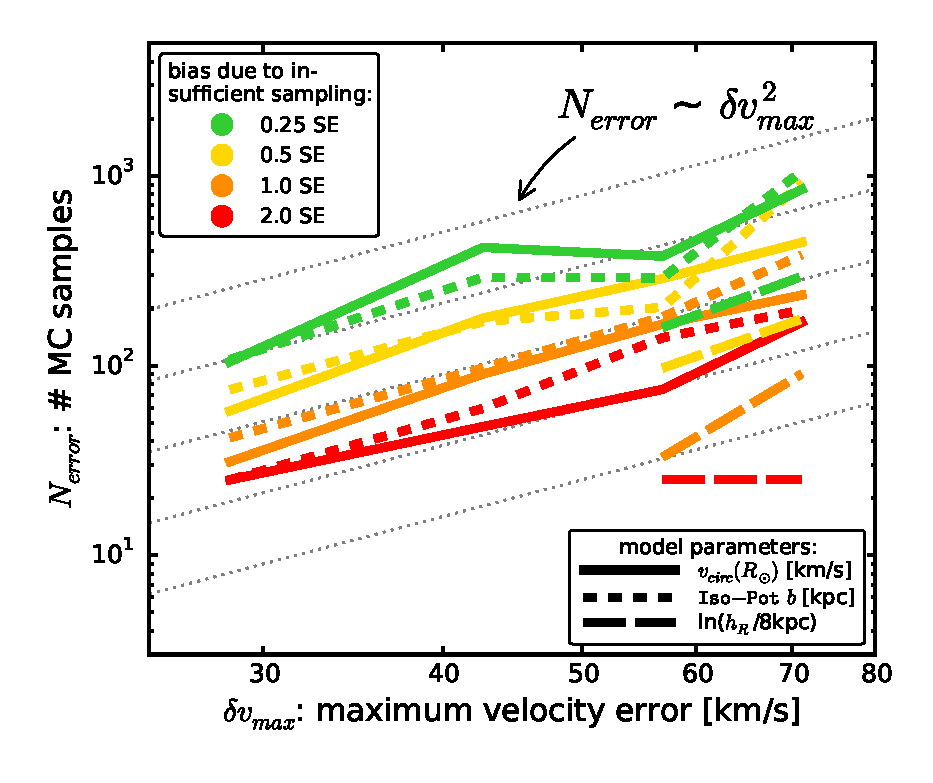
\includegraphics[width=\columnwidth]{figs/isoSphFlexErrConv_MC_vs_error_2.eps}
\caption{Number of MC samples $N_\text{samples}$ needed for the numerical convolution of the model probability with the measurement uncertainties in Equation \ref{eq:errorconv}, given the maximum velocity uncertainty $\delta v_\text{max}$ within the stellar sample with respect to the sample's kinematic temperature $\bar{\sigma}$. Insufficient sampling introduces systematic biases in the parameter recovery---the size of the bias is indicated in the legend. The relation found here, $N_\text{samples} \propto \delta v_\text{max}^2$, was distilled from analyses of mock data sets with different proper motion uncertainties $\delta \mu \in [2,5]~\text{mas yr}^{-1}$ in the absence of position uncertainties (see Test \ref{test:isoSphFlexErrConv_MC_vs_error} in Table \ref{tbl:tests}). The proper motion uncertainty $\delta \mu$ translates to heteroscedastic velocity uncertainties according to $\delta v [\text{km s}^{-1}] \equiv 4.74047 \cdot r[\text{kpc}] \cdot \delta \mu [\text{mas yr}^{-1}]$, with $r$ being the distance of the star from the Sun. Stars with larger $\delta v$ require more $N_\text{samples}$ for the integral over its measurement uncertainties to converge; we therefore show how the $N_\text{samples}$---needed for the \pdf{} of the \emph{whole} data set to be converged---depends on the \emph{largest} velocity error $\delta v_\text{max} \equiv \delta v(r_\text{max})$ within the data set. We used $N_\text{samples} = 800$ and  $1200$ for $\delta \mu \leq 3~\text{mas yr}^{-1}$ and $\delta \mu > 3~\text{mas yr}^{-1}$, respectively, as the reference for the converged convolution integral (see also left panels in Figure \ref{fig:isoSphFlexErrConv_bias_vs_SE}). We plot $\delta v_\text{max}$ in units of the sample temperature, which we quantify by $\bar{\sigma} \equiv (\sigma_{R,0} + \sigma_{z,0})/2$ (see Table \ref{tbl:referenceMAPs} for the \texttt{hot} qDF). This figure was generated from mock data sets with $N_{*}=10,000$. We found that for $N_{*}=5,000$ the required $N_\text{samples}$ remains similar for $b$, but gets smaller for $v_\text{circ}(R_\odot)$. Overall we expect that we need less accuracy and therefore smaller $N_\text{samples}$ for smaller $N_{*}$. \Wilma{[TO DO: some of the 25 MC sample analyses have to be re-done.]}}
\label{fig:isoSphFlexErrConv_MC_vs_error}
\end{figure}

%=============================================================

%====================================================================

%FIGURE: Triangle plot, shape of likelihood, multi-variate Gaussian

\begin{figure*}[!htbp]
\centering
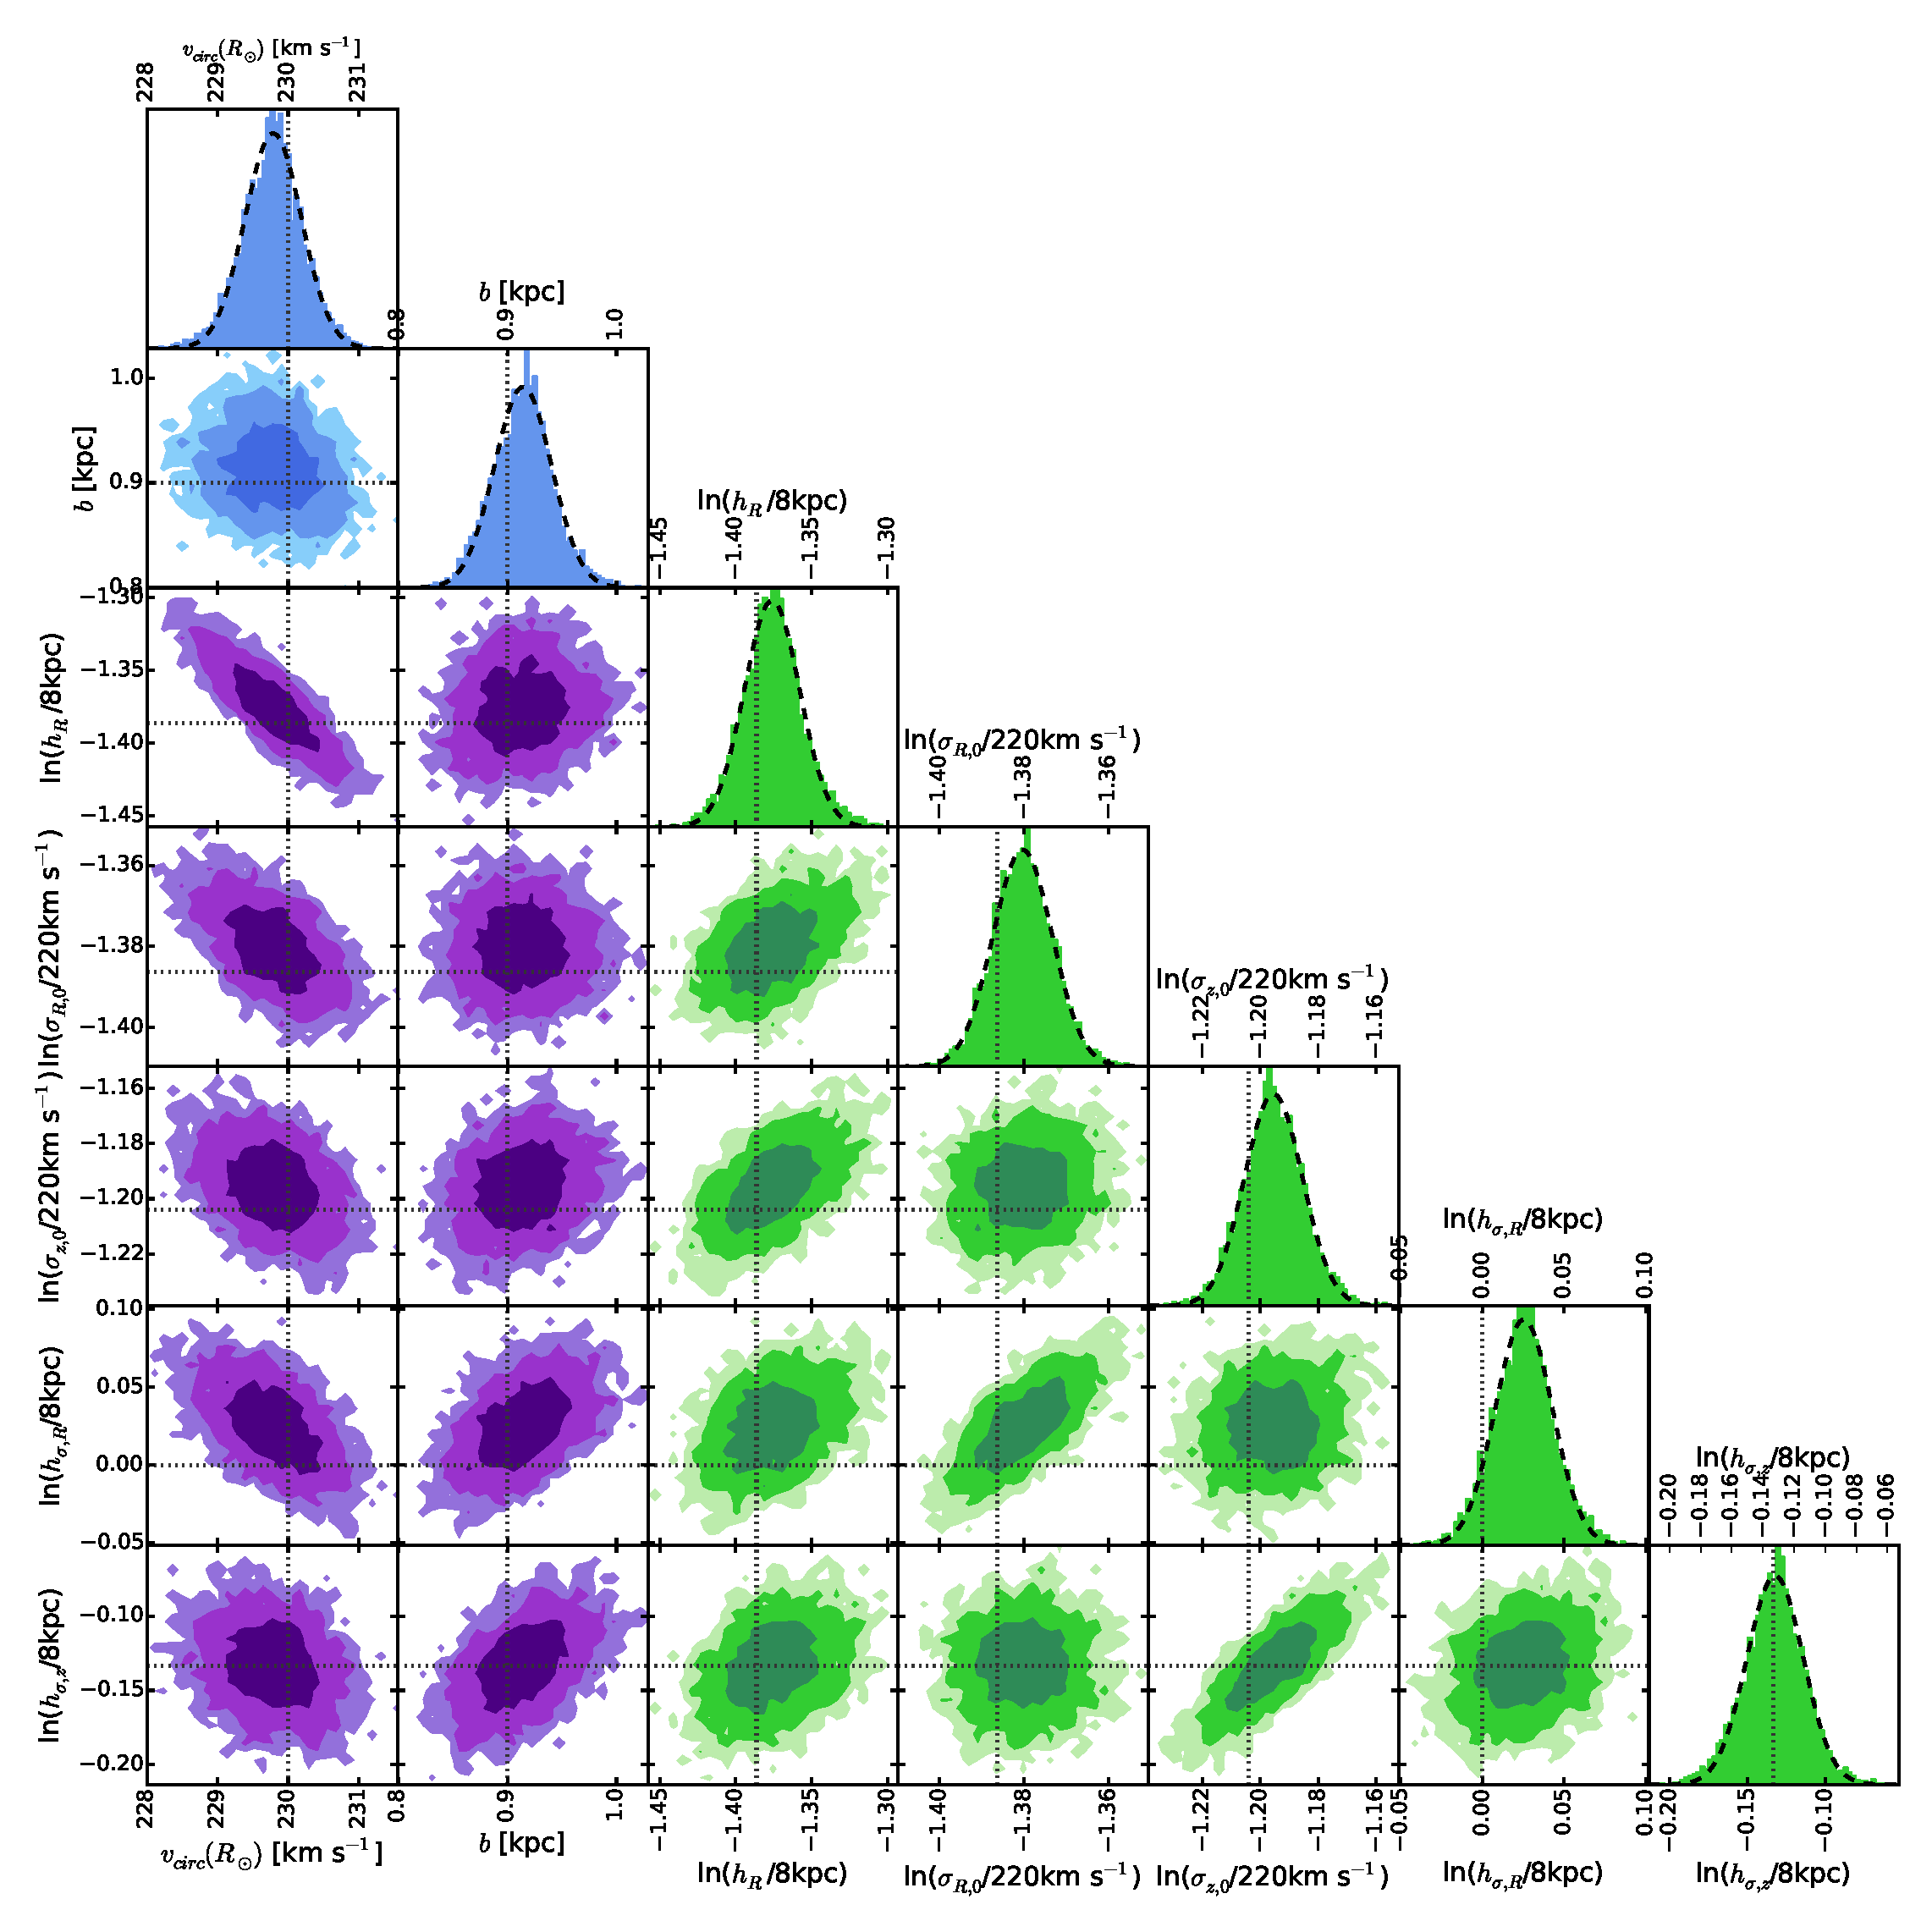
\includegraphics[width=0.7\textwidth]{figs/isoSphFlex_short_hot_2kpc_triangle_MCMC.eps}
\caption{The \pdf{} (proportional to the likelihood in Equation \ref{eq:prob}) in the parameter space $\pmodel{} = \{p_\Phi,p_\text{DF}\}$ for one example mock data set (see Test \ref{test:isoSphFlex} in Table \ref{tbl:tests}). Blue indicates the \pdf{} for the potential parameters, green the qDF parameters. The true parameters are marked by dotted lines. The dark, medium and bright contours in the 2D distributions represent 1, 2 and 3 sigma confidence regions, respectively. The parameters are weakly to moderately covariant, but their level of covariance depends on the actual choice of the mock data's \pmodel{}. The \pdf{} here was sampled using MCMC. The dashed lines in the 1D distributions are Gaussian fits to the histogram of MCMC samples. This demonstrates very well that for such a large number of stars, the \pdf{} approaches the shape of a multi-variate Gaussian, as expected for an maximum likelihood estimator. \Wilma{[TO DO: $\text{km s}^{-1}$]}}
\label{fig:isoSphFlex_triangleplot}
\end{figure*}

%====================================================================


\subsection{Data likelihood} \label{sec:likelihood}


As data $D$ we consider here the positions and velocities of a sub-population of stars within a given survey selection function $\text{SF}(\vect{x})$,
\begin{eqnarray*}
D  \equiv \{ \vect{x}_i,\vect{v}_i \mid && \text{(star $i$ being in given sub-population)}\nonumber\\
&\wedge& (\text{SF}(\vect{x}_i) > 0) \}.
\end{eqnarray*}

We fit a model potential and DF (here: the qDF) which are specified by a number of fixed and free model parameters,
\begin{eqnarray*}
\pmodel \equiv \{ p_\text{DF} , p_\Phi \}.
\end{eqnarray*}
The orbit of the $i$-th star in a potential with $p_\Phi$ is labeled by the actions $\vect{J}_i := \vect{J}[\vect{x}_i,\vect{v}_i\mid p_{\Phi}]$ and the DF evaluated for the $i$-th star is then $\text{DF}(\vect{J}_i \mid \pmodel) := \text{DF}(\vect{J}[\vect{x}_i,\vect{v}_i\mid p_{\Phi}] \mid p_\text{DF})$.

The likelihood of the data given the model is, following BR13,
\begin{eqnarray}
&&\mathscr{L}(D \mid \pmodel) \nonumber\\
&&\equiv \prod_i^{N_*} p(\vect{x}_i,\vect{v}_i \mid \pmodel) \nonumber\\
&&= \prod_i^{N_*} \frac{\text{DF}(\vect{J}_i \mid \pmodel) \cdot \text{SF}(\vect{x}_i)}{\int \Diff 3 x \Diff 3 v \  \text{DF}(\vect{J} \mid \pmodel) \cdot \text{SF}(\vect{x})}\nonumber\\
&&\propto \prod_i^{N_*} \frac{\text{DF}(\vect{J}_i \mid \pmodel)}{\int \Diff 3 x \  \rho_\text{DF}(R,|z| \mid \pmodel) \cdot \text{SF}(\vect{x})}, \label{eq:prob}
%\label{eq:likelihood}
\end{eqnarray}
where $N_*$ is the number of stars in $D$, and in the last step we used Equation \ref{eq:tracerdensity}. $\prod_i\text{SF}(\vect{x}_i)$ is independent of \pmodel{}, so we treat it as unimportant proportionality factor. We find the best fitting \pmodel{} by maximizing the posterior probability distribution $\pdf{}(\pmodel \mid D)$, which is, according to Bayes' theorem, proportional to the likelihood $\mathscr{L}(D\mid \pmodel)$ times a prior $p(\pmodel)$. We assume flat priors in both $p_\Phi$ and
\begin{eqnarray}
p_\text{DF} := \{ \ln h_R, \ln \sigma_{R,0}, \ln \sigma_{z,0}, \ln h_{\sigma,R}, \ln h_{\sigma,z} \} \label{eq:p_DF}
\end{eqnarray}
(see Section \ref{sec:qDF}) throughout this work. Then \pdf{} and likelihood are proportional to each other and differ only in units.

The normalisation in Equation \ref{eq:prob} is a measure for the total number of tracers inside the survey volume,
\begin{equation}
M_\text{tot} \equiv \int \Diff 3 x \  \rho_\text{DF}(R,|z| \mid \pmodel) \cdot \text{SF}(\vect{x}).\label{eq:normalisation}
\end{equation}
In the case of an axisymmetric Galaxy model and $\text{SF}(\vect{x})=1$ within the observation volume (as in most tests in this work), the normalisation is essentially a two-dimensional integral in the $R$-$z$ plane over $\rho_{DF}$ with finite integration limits. We evaluate the integrals using Gauss-Legendre quadratures of order 40. The integral over the azimuthal direction can be solved analytically. 
\Wilma{[TO DO: Write normalisation everywhere in the same waz.]}

It turns out that a sufficiently accurate evaluation of the likelihood is computationally expensive, even for only one set of model parameters. This expense is dominated by the number of action calculations required, which in turn depends on $N_*$ and the numerical accuracy of the tracer density interpolation grid with $N_x^2+N_v^3$ grid points in Equation \ref{eq:tracerdensity} needed for the likelihood normalization in Equation \ref{eq:normalisation}. The accuracy of the normalization has to be chosen high enough, such that the resulting numerical error 
\begin{equation}
\delta_{M_\text{tot}} \equiv \frac{M_\text{tot,approx}(N_x,N_v,n_\sigma) -  M_\text{tot} }{M_\text{tot}}\label{eq:relerrlikelihood}
\end{equation}
does not dominate the numerically calculated log-likelihood, i.e.,
\begin{eqnarray}
& &\log \mathscr{L}_\text{approx}(D \mid \pmodel) \nonumber\\
&& = \sum_i^{N_*} \log \text{DF}(\vect{J_i} \mid \pmodel) - N_* \log(M_\text{tot})\nonumber\\
&& - N_* \log (1 + \delta_{M_\text{tot}}),\label{eq:loglikelihood_relerr}
\end{eqnarray}
with
\begin{eqnarray}
N_* \log (1 + \delta_{M_\text{tot}}) \leq 1.\nonumber
\end{eqnarray}
Otherwise numerical inaccuracies could lead to systematic biases in the potential and DF recovery. For data sets as large as $N_* = 20,000$ stars, which in the age of Gaia could very well be the case \HW{[TO DO: Really???]}, one needs a numerical accuracy of 0.005\% in the normalisation. Figure \ref{fig:norm_accuracy} demonstrates that the numerical accuracy we use in the analysis, $N_x=16$, $N_v=24$ and $n_\sigma=5$, does satisfy this requirement. This is slightly higher than in BR13, where $N_* \sim 100$ \Wilma{[TO DO: CHECK]}.\\


%====================================================================

Measurement uncertainties of the data have to be incorporated in the likelihood. We assume Gaussian uncertainties in the observable space $\vect{y} \equiv (\tilde{\vect{x}},\tilde{\vect{v}})=(\text{RA},\text{Dec},(m-M),\mu_\text{RA} \cdot \cos \text{Dec},\mu_\text{Dec},v_\text{los})$, i.e., the $i$-th star's observed $\vect{y}_i$ are drawn from the normal distribution $N[{\vect{y}'}_i,\delta \vect{y}_i]$, with ${\vect{y}_i}'$ being the star's true phase-space position and $\delta \vect{y}_i$ its uncertainty . Stars follow the distribution function (DF$(\vect{y}') \equiv$ DF$(\vect{J}[\vect{y}' \mid p_\Phi] \mid p_\text{DF})$ for short), convolved with the measurement uncertainties $N[0,\delta \vect{y}]$ \Wilma{[TO DO: CHECK AGAIN]}. The selection function SF$(\vect{y})$ acts on the space of (error affected) observables. Then the probability of one star becomes
\begin{eqnarray*}
&&\tilde{p}(\vect{y}_i \mid p_\Phi,p_\text{DF},\delta \vect{y}_i)\\
& \equiv& \frac{\text{SF}(\vect{y}_i) \cdot \int \Diff{6} y' \  \text{DF}(\vect{y}') \cdot N[\vect{y}_i,\delta \vect{y}_i]}{\int \Diff{6}y'  \  \text{DF}(\vect{y}')  \cdot  \int \Diff{6} y \  \text{SF}(\vect{y})  \cdot N[\vect{y}',\delta \vect{y}_i]}.
\end{eqnarray*}
In the case of uncertainties in distance or (RA,Dec), the evaluation of this is computational expensive - especially if the stars have heteroscedastic $\delta \vect{y}_i$. In practice we apply the following approximation,
\begin{eqnarray}
&&\tilde{p}(\vect{y}_i \mid p_\Phi,p_\text{DF},\delta \vect{y}_i) \nonumber\\
&&\approx \frac{ \text{SF}(\vect{x}_i)}{M_\text{tot}} \cdot \frac{1}{N_\text{samples}} \sum_n^{N_\text{samples}}  \text{DF}(\vect{x}_i,\vect{v}[\vect{y}'_{i,n}]) \label{eq:errorconv}
\end{eqnarray}
with
\begin{eqnarray}
\vect{y}'_{i,n} \sim N[\vect{y}_i,\delta \vect{y}_i]\nonumber
\end{eqnarray}
We calculate the convolution using Monte Carlo (MC) integration with $N_\text{samples}$ samples. The above approximation assumes that the star's \emph{position} $\vect{x}_i$ is perfectly measured. As the selection function is also velocity independent, this simplifies the normalisation drastically to Equation \ref{eq:normalisation}. Measurement uncertainties in $\mathrm{RA}$ and $\mathrm{Dec}$ are often negligible anyway. The uncertainties in the Galactocentric \emph{velocities} $\vect{v}_i = (v_{R,i},v_{T,i},v_{z,i})$ depend besides on $\delta \vect{\mu}$ and $\delta v_\text{los}$ also on the distance and its uncertainty, which we do \emph{not} neglect when drawing MC samples $\vect{y}'_{i,n}$ from the full uncertainty distribution $N[\vect{y}_i,\delta \vect{y}_i]$. Figure \ref{fig:isoSphFlexErrConv_MC_vs_error} demonstrates that in the absence of position uncertainties the $N_\text{samples}$ needed for the convolution integral to converge depends as
\begin{equation*}
N_\text{samples} \propto \delta v^2
\end{equation*}
on the uncertainties in the (1D) velocities. We found that the required $N_\text{samples}$ to reach a given accuracy does not depend strongly on the number of stars in the sample. But in general we expect that we need higher accuracy and therefore more $N_\text{samples}$ for larger data sets.
\\A similar but only one-dimensional treatment of measurement uncertainties in $v_z$ was already applied by BR13.


%\subsection{Fitting procedure} \label{sec:fitting}

To search the $(p_\Phi,p_\text{DF})$ parameter space for the maximum of the \pdf{} in Equation \ref{eq:normalisation}, we go beyond the single fixed grid search by BR13 and employ an effective two-step procedure: Nested-grid search and Monte-Carlo Markov Chain.

The first step employs a nested-grid search to find the approximate peak and width of the \pdf{} in the high-dimensional \pmodel{}  space at a low number of likelihood evaluations.

\begin{itemize}
\item \emph{Initialization.} For $N_p$ free model parameters \pmodel{}, we start with a sufficiently large grid with $3^N_p$ regular points.

\item  \emph{Evaluation.} We evaluate the \pdf{} at each grid-point similar to BR13 (their Figure 9):  An outer loop iterates over the potential parameters $p_\Phi$ and pre-calculates all $N_* \times N_\text{samples} + N_x^2 \times N_v^3$ actions (\# stars times \# MC samples for convolution with measurement uncertainties, plus actions required for density interpolation grid in Equation \ref{eq:tracerdensity}). Then an inner loop evaluates Equation \ref{eq:normalisation} for all DF parameters $p_\text{DF}$ in the given potential.

\item \emph{Iteration.} For each of the model parameters \pmodel{}, we marginalize the \pdf{}. A Gaussian is fitted to the marginalized \pdf{} and the peak $\pm ~ 4$ sigma become the boundaries of the next $3^{N_p}$ grid. The grid might be still too coarse or badly positioned to fit Gaussians. In that case, we either zoom into the grid point with the highest probability or shift the current range to find new approximate grid boundaries. We proceed with iteratively evaluating the \pdf{} on finer and finer grids, until we have found a reliable 4-sigma fit range in each of the \pmodel{} dimensions. The central grid point is then very close to the best fit \pmodel{}, and the grid range is of the order of the \pdf{} width.

\item \emph{The fiducial qDF.} To save time by pre-calculating actions, they have to be independent of the choice of $p_\text{DF}$. However, the normalisation in Equation \ref{eq:normalisation} requires actions on a $N_x^2 \times N_v^3$ grid and the grid range in velocity space \emph{do} depend on the current $p_\text{DF}$ (see Equation \ref{eq:tracerdensity}). To relax this, we follow BR13 and use a fixed set of qDF parameters (the \emph{fiducial qDF}) to set the velocity grid boundaries in Equation \ref{eq:tracerdensity} globally for a given $p_\Phi$. Choosing a fiducial qDF that is very different from the true DF can however lead to large biases in the \pmodel{} recovery. BR13 did not account for that. \RM{} avoids this as follows: To get successively closer to the optimal fiducial qDF---the (yet unknown) best fit $p_\text{DF}$---we use in each iteration step of the nested-grid search the central grid point of the current \pmodel{} grid as the fiducial qDF.  As the nested-grid search approaches the best fit values, the fiducial qDF approaches its optimum as well. 

\item \emph{Computational expense.} Overall the computation speed of this nested-grid approach is dominated (in descending order of importance) by a) the complexity of potential and action calculation, b) the $N_* \times N_\text{samples} + N_x^2 \times N_v^3$ actions required to be calculated per $p_\Phi$, c) the number of potential parameters and d) the number of DF parameters.
\end{itemize}

The second step samples the shape of the \pdf{} using a Monte-Carlo Markov Chain (MCMC). Formally, calculating the \pdf{} on a fine grid like BR13 (e.g., with $K=11$ grid points in each dimension) would provide the same information. However the number of expensive \pdf{} evaluations scales as $K^{N_p}$. For a high-dimensional \pmodel{} ($N_p>4$), a MCMC approach might sample the \pdf{} much faster: We use \emph{emcee} by \citet{2013PASP..125..306F} and release the walkers very close to the best fit \pmodel{} found by the nested-grid search, which assures fast convergence in much less than $K^{N_p}$ \pdf{} evaluations. We also use the best fit \pmodel{} of the grid-search as fiducial qDF for the whole MCMC. In doing so, the normalisation varies smoothly with different $\pmodel{}$ and is slightly less sensitive to the accuracy in Equation \ref{eq:tracerdensity}.
%%-----------------------------------------------------------------------------------------------------------------------------------------------------------------------------
%
%%-----------------------------------------------------------------------------------------------------------------------------------------------------------------------------
%%Results
%\section{Results} \label{sec:results}

We are now in a position to explore the limitations of action based modelling posed in the introduction: (i) unbiased estimates; (ii) survey volume; (iii) imperfect selection function; (iv) measurement errors; (v) actual DF or (vi) Potential not spanned by the space of models. We do not explore the breakdown of the assumption that the system is axisymmetric and
in steady state. With the exception of the test suite on measurement errors in \S\ref{sec:results_errors}, we assume that the phase-space errors are negligible. All tests are also summarized in Table \ref{tbl:tests}. 

\HW{[TO DO: Hans-Walter said that there are diagnostic plots in this papers that can be eliminated and their essence summarized in 1-2 sentences in the text. Fine. But which plots does he think can be eliminated? My plots contain either results or are only there to make the paper more readable for others.]}




%\subsection{Model parameter estimates in the limit of large data sets} \label{sec:largedata}

The individual \MAP{}s in BR13 contained typically between 100 and 800 objects, so that each \MAP{} implied a quite broad \pdf{} for the model parameters $\pmodel{}$. Here we explore what happens in the limit of much larger samples, say $N_{*} = 20,000$ objects.  As outlined in Section \ref{sec:likelihood}, the immediate consequence of larger samples is given by the likelihood normalization requirement $\log(1+\delta M_\text{tot})\le 1/N_{*}$ (Equation \ref{eq:accuracycondition}), which is the modelling aspect that drives the computing time. This issues aside, we would however expect that in the limit of large data sets with vanishing measurement uncertainties the \pdf{}s of the \pmodel{} become Gaussian, with a \pdf{} width (i.e., the standard error (SE) on the parameter estimate) that scales as $1/\sqrt{N_{*}}$. Further, we must verify that any bias in the \pdf{} expectation value is considerably less than the error, even for quite large samples.

%====================================================================

%FIGURE: width of likelihood propto 1/sqrt(N)

\begin{figure}[!htbp]
\plotone{figs/sqrtNiso_Stddev_Vs_N.eps}
\caption{The width of the \pdf{} (see Equation \ref{eq:prob}) for two fit parameters found from analyses of 132 mock data sets vs. the number of stars in each data set, $N_{*}$. (The mock data was created according to the model parameters given in Test \ref{test:sqrtNiso} in Table \ref{tbl:tests}.) The relative standard error (SE) was found from a Gaussian fit to the marginalized \pdf{} for each model parameter. As can be seen, for large data samples the width of the \pdf{} scales with $1/\sqrt{N_{*}}$ as expected.} 
\label{fig:sqrtNiso}
\end{figure}

%====================================================================

%====================================================================

%FIGURE: central limit theorem is satisfied

\begin{figure}[!htbp]
\centering
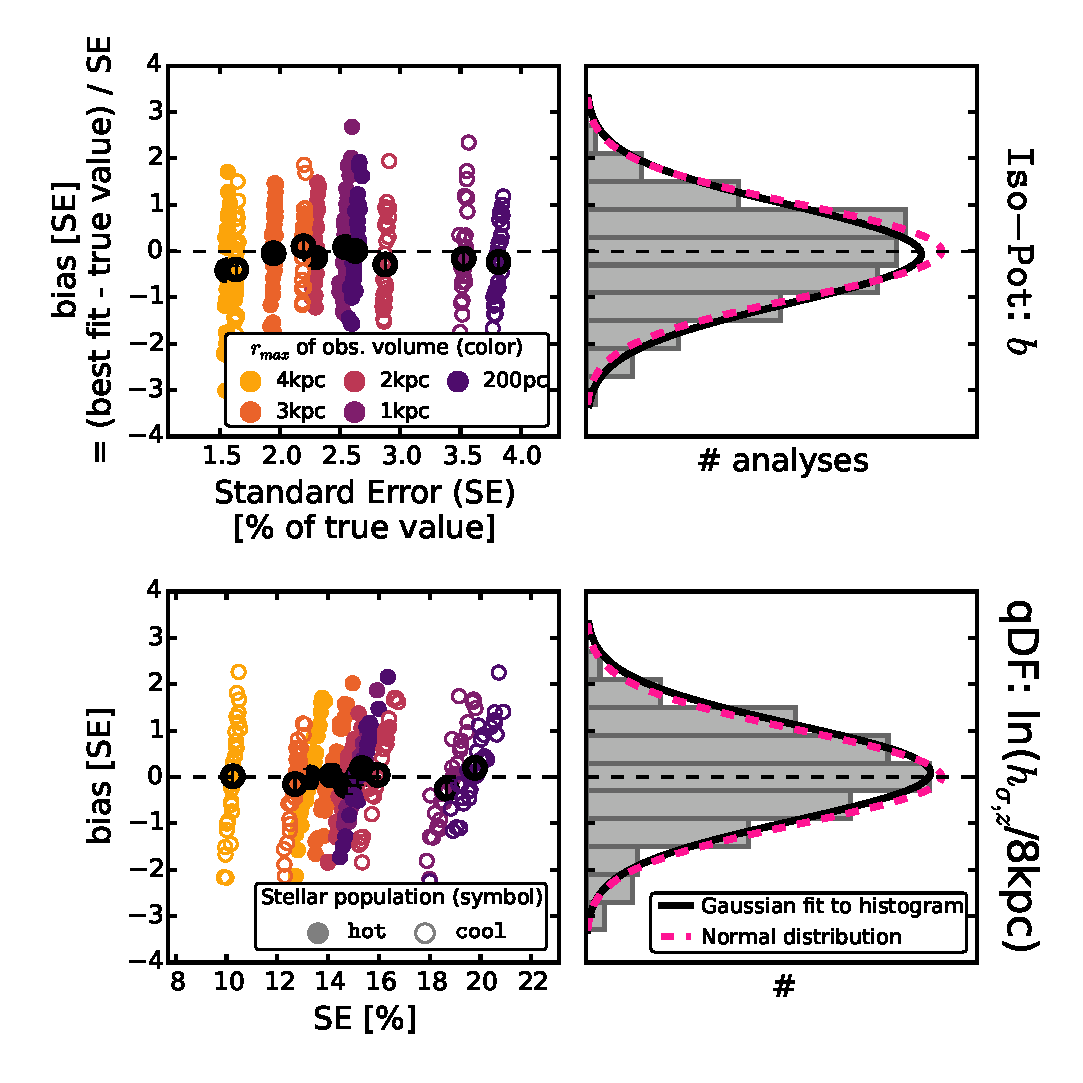
\includegraphics[width=\columnwidth]{figs/isoSph_CLT_2.eps}
\caption{(Un-)bias of the parameter estimates. Maximum likelihood estimators converge to the true parameter values for large numbers of data points and have a Gaussian spread---if the model assumptions are fulfilled. To test that these conditions are satisfied for \RM{}, we create 320 mock data sets, which come from two different stellar populations and five spherical observation volumes (see legends). (All model parameters are summarized in Table \ref{tbl:tests} as Test \ref{test:isoSph_CLT}.) Bias and relative standard error (SE) are derived from the marginalized \pdf{} for two model parameters (isochrone scale length $b$ in the first row and qDF parameter $h_{\sigma,z}$ in the second row). The second column displays a histogram of the 320 bias offsets. As it closely follows a Normal distribution, our modelling method is therefore well-behaved and unbiased. The black dots denote the \pdf{} expectation value for the 32 analyses belonging to the same $\pmodel{}$.}
\label{fig:isoSph_CLT}
\end{figure}

%====================================================================

%====================================================================

%FIGURE: Does shape and position of obs. volume matter?


\begin{figure}[!htbp]
\centering
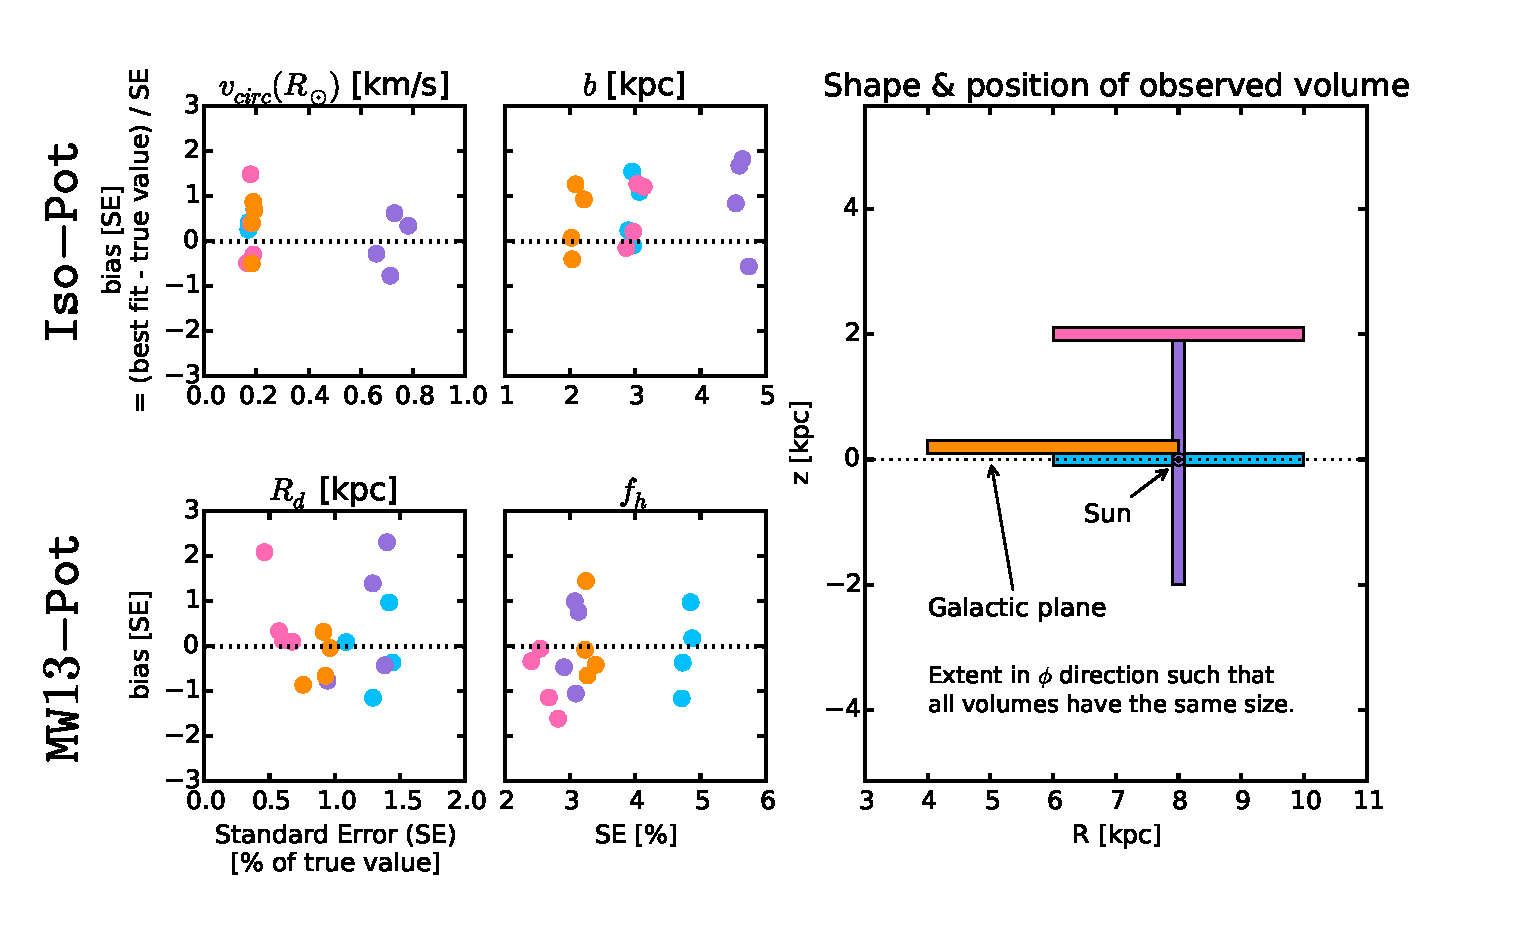
\includegraphics[width=\columnwidth]{figs/wedFlexVol_bias_vs_SE.eps}
\caption{Bias vs. standard error in recovering the potential parameters for mock data sets drawn from four different wedge-shaped test observation volumes within the Galaxy (illustrated in the upper panel; the corresponding analyses are colour-coded) and two different potentials (\texttt{Iso-Pot} and \texttt{MW13-Pot} from Table \ref{tbl:referencepotentials}; see also Test \ref{test:wedFlexVol} in Table \ref{tbl:tests} for all model parameters used). Standard error and offset were determined from a Gaussian fit to the marginalized \pdf{}. The angular extent of each wedge-shaped observation volume was adapted such that all have a volume of $4.5~\text{kpc}^3$, even though their extent in $(R,z)$ is different. Overall there is no clear trend that an observation volume around the Sun, above the disk or at smaller Galactocentric radii should give remarkably better constraints on the potential than the other volumes.}
\label{fig:wedFlexVol_bias_vs_SE}
\end{figure}


%====================================================================

Using sets of mock data, created according to the procedure in Section \ref{sec:mockdata} and a fiducial model for \pmodel{} (see Table \ref{tbl:tests}, Tests \ref{test:sqrtNiso}, \ref{test:isoSph_CLT}, and \ref{test:isoSphFlex}), we verified that \RM{} satisfies all these conditions and expectations: Figure \ref{fig:isoSphFlex_triangleplot} illustrates the joint \pdf{}s of all \pmodel{}. The \pdf{} is a multivariate Gaussian that projects into Gaussians when considering the marginalized \pdf{} for all the individual \pmodel{}. Figure \ref{fig:sqrtNiso} then demonstrates that the \pdf{} width indeed scales as $1/\sqrt{N_{*}}$. Figure \ref{fig:isoSph_CLT} illustrates even more that \RM{} behaves like an unbiased maximum likelihood estimator: The average parameter estimates from many mock samples with identical underlying \pmodel{} are very close to the input \pmodel{}, and the distribution of the actual parameter estimates are a Gaussian around it. 
%\subsection{The Role of the Survey Volume Geometry} \label{sec:results_obsvolume}

\Wilma{[TO DO: Mach einheitlich, wie die Tests in Captions und Text erwähnt werden (in Klammer)]}

To explore the role of the survey volume at given sample size, we devise two suites of mock data sets: 

The first suite draws mock data from the same \pmodel{}, two different potentials (\texttt{Iso-Pot} and \texttt{MW13-Pot}, see Test \ref{test:wedFlexVol} in Table \ref{tbl:tests}), and volume wedges (see Section \ref{sec:selectionfunction}) at {\it different positions within the Galaxy}, illustrated in the right upper panel of Figure \ref{fig:wedFlexVol_bias_vs_SE}. To isolate the role of the survey volume geometry, the mock data sets are equally large ($N_{*} = 20,000$) in all cases, and are drawn from identical total survey volumes ($4.5~\text{kpc}^3$, achieved by adjusting the angular width of the wedges). The results are shown in Figure \ref{fig:wedFlexVol_bias_vs_SE}.
\\The second suite of mock data sets was already introduced in Section \ref{sec:largedata} (see also Test \ref{test:isoSph_CLT} in Table \ref{tbl:tests}), where mock data sets were drawn from five spherical volumes around the Sun with different maximum radius, for two different stellar populations. The results of this second suite are shown in Figure \ref{fig:isoSph_CLT} and demonstrate the effect of the {\it size of the survey volume}.

Figure \ref{fig:isoSph_CLT} demonstrates that, given a choice of $p_\text{DF}$, a larger volume always results in tighter constraints. There is no obvious trend that a hotter or cooler population will always give better results \Wilma{[TO DO: Comment from HW: The question of whether a hotter or a colder population gives tighter constraints is an important question, but it seems buries here in a section that is dedicated to another matter, namely the question of volume ... It's OK to leave it here, but somewhere we need to say clearly: whether the population is hot or cold does not make a big and generic difference...]}; it depends on the survey volume and the model parameter in question. In Figure \ref{fig:wedFlexVol_bias_vs_SE} the wedges all have the same volume and all give results of similar precision. Minor differences (e.g., the \texttt{Iso-Pot} potential being less constrained in the wedge with large vertical but small radial extent) are a special property of the considered potential and parameters, and not a global property of the corresponding survey volume. In the case of an axisymmetric model galaxy, the extent in $\phi$ direction is not expected to matter. Overall radial extent and vertical extent seem to be equally important to constrain the potential. In addition Figure \ref{fig:wedFlexVol_bias_vs_SE} implies that for these cases volume offsets in the radial or vertical direction have at most a modest impact - even in case of the very large sample size at hand.

While it appears that the argument for significant radial and vertical extent is generic, we have not done a full exploration of all combinations of \pmodel{} and volumina.

%====================================================================

%FIGURE: Does shape and position of obs. volume matter?


\begin{figure*}[!htbp]
\centering
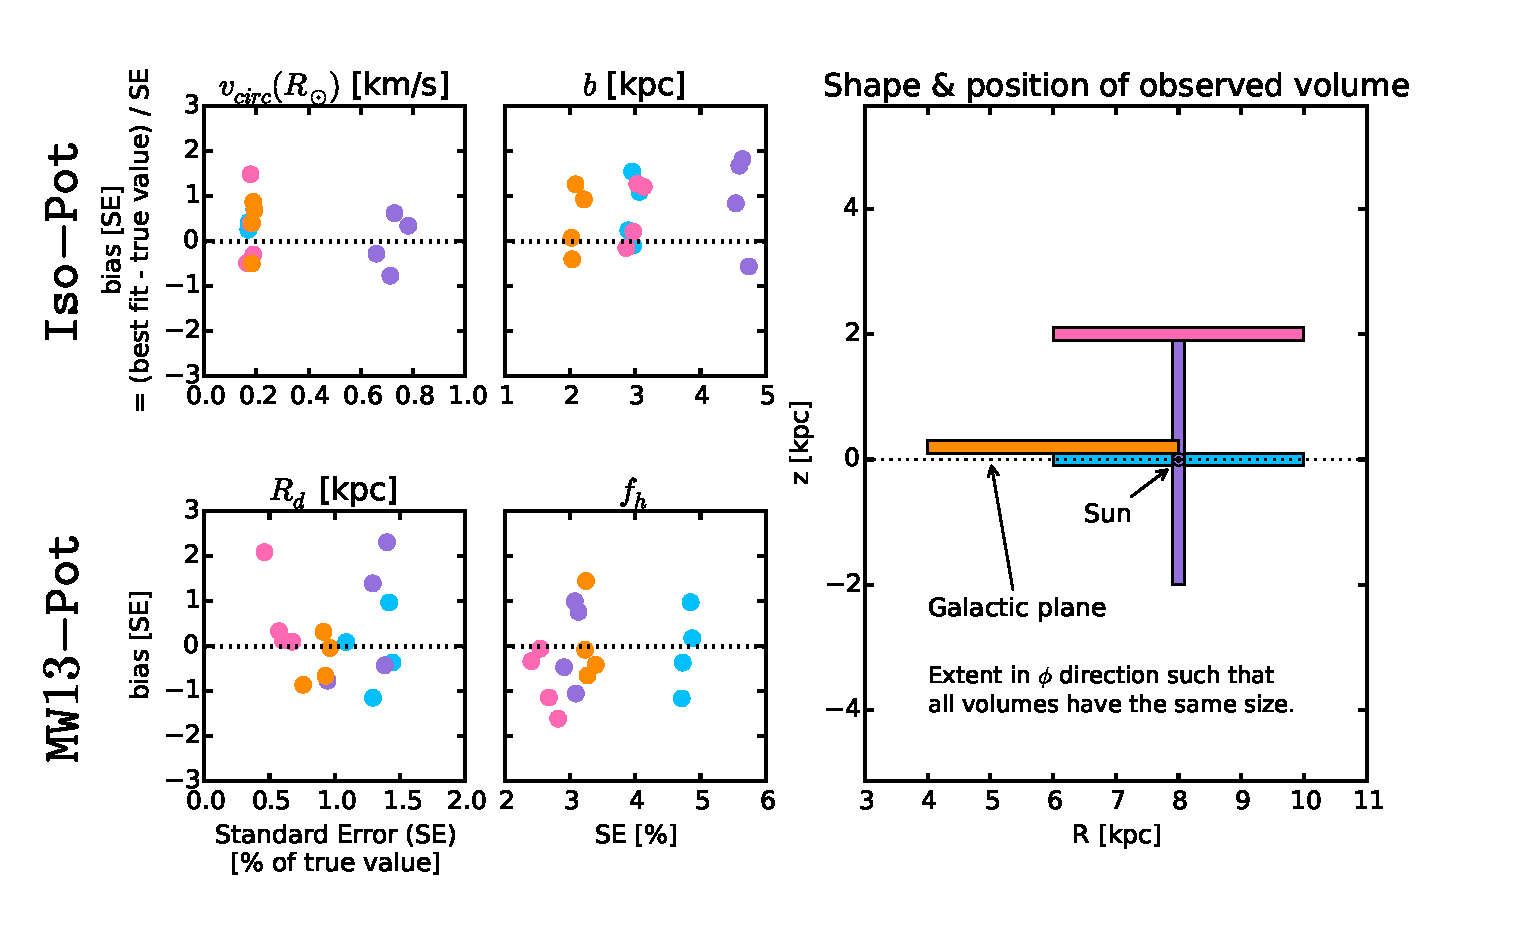
\includegraphics[width=0.7\textwidth]{figs/wedFlexVol_bias_vs_SE.eps}
\caption{Bias vs. standard error in recovering the potential parameters for mock data stars drawn from four different wedge-shaped test observation volumes within the Galaxy (illustrated in the right panel; the corresponding analyses are colour-coded) and two different potentials (\texttt{Iso-Pot} and \texttt{MW13-Pot} from Table \ref{tbl:referencepotentials}; see also Test \ref{test:wedFlexVol} in Table \ref{tbl:tests} for all model parameters used). Standard error and offset were determined from a Gaussian fit to the marginalized \pdf{}. The angular extent of each wedge-shaped observation volume was adapted such that all have the volume of $4.5 \text{ kpc}^3$, even though their extent in $(R,z)$ is different. Overall there is no clear trend, that an observation volume around the Sun, above the disk or at smaller Galactocentric radii should give remarkably better constraints on the potential than the other volumes. \Wilma{[TO DO: Write in Plot "... that all wedges have the same volume".] [TO DO: No units in parameters in titles]}}
\label{fig:wedFlexVol_bias_vs_SE}
\end{figure*}


%====================================================================

%\subsection{Impact of Misjudging the Completeness of the Data Set} \label{sec:results_incompR}

The selection function (see Section \ref{sec:selectionfunction}) can be very complex and is therefore sometimes not perfectly known. Here we investigate how much this could affect the recovery of the potential. We do this by creating mock data in a spherical survey volume around the Sun with a spatially varying incompleteness function, while assuming constant completeness in the \RM{} analysis. Our test case uses a completeness function which drops linearly with distance $r$ from the Sun (see Test \ref{test:isoSphFlexIncomp} in Table \ref{tbl:tests} and Figure \ref{fig:isoSphFlexIncomp_completeness_shapes}). This captures the relevant case of stars being less likely to be observed (than assumed) the further away they are (e.g. due to unknown dust obscuration). 

Figure \ref{fig:isoSphFlexIncompR_violins} demonstrates that the potential recovery with \RM{} is very robust against somewhat wrong assumptions about the radial completeness of the data. The robustness for the \texttt{cool} stellar population is even more striking than for the \texttt{hot} population. The reason for this robustness could be, that much information about the potential comes from the rotation curve measurements in the plane, which is not affected by the incompleteness of the sample. We test this by not including tangential velocity measurements in the analysis of the data sets from Figure \ref{fig:isoSphFlexIncompR_violins} (by marginalizing the likelihood in Equation \ref{eq:prob} over $v_T$). Figure \ref{fig:isoSphFlexIncompR_marginal_violins} shows that in this case the potential is much less tightly constrained, even for 20,000 stars. For only small deviations of true and assumed completeness ($\lesssim 10\%$) we can however still incorporate the true potential in our fitting result (see Figure \ref{fig:isoSphFlexIncomp_marginal_violins}).

We found similar results also for spatial incompleteness functions varying with $z$

\HW{[TO DO: Comment by HW: I don't have an immediate solution for this, but again, it seems the interesting question of "how much of the information is in the rotation curve" is 'hidden' in the section on selection functions... - What does he mean by that?]}


%=============================



%FIGURE: isoSphFlexIncompR in mock data space

\begin{figure}[!htbp]
\centering
\includegraphics[width=0.7\columnwidth]{figs/isoSphFlexIncompR_completeness_shapes.eps}
\caption{Illustration of the selection function used to investigate the impact of misjudgements of the radial incompleteness of the data in Figure \ref{fig:isoSphFlexIncompR_violins}. The survey volume is a sphere around the Sun and the percentage of observed stars is decreasing linearly with radius from the Sun. How fast this detection/incompleteness rate drops is quantified by the factor $\epsilon_r$.} 
\label{fig:isoSphFlexIncompR_completeness_shapes}
\end{figure}

%FIGURE: isoSphFlexIncompR

\begin{figure}[!htbp]
\centering
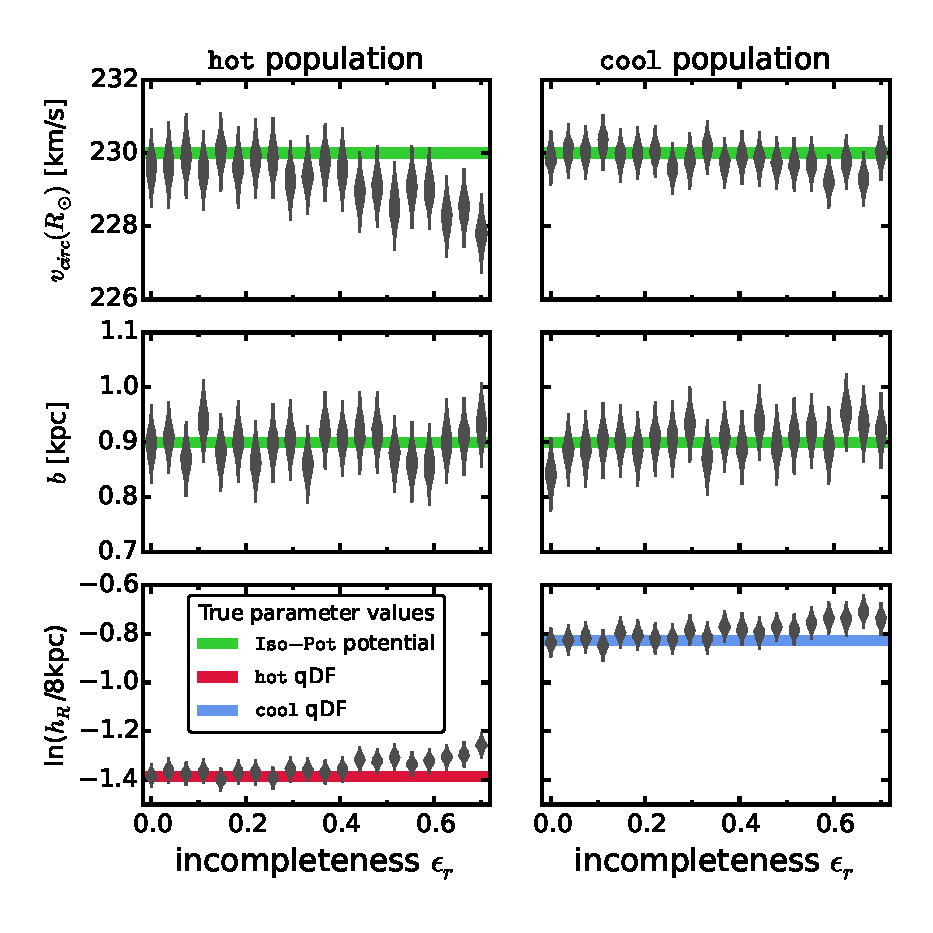
\includegraphics[width=\columnwidth]{figs/isoSphFlexIncompR_violins_2.eps}
\caption{Influence of wrong assumptions about the radial incompleteness of the data on the parameter recovery with \RM{}. Each mock data set was created with different incompleteness parameters $\epsilon_r$ (shown on the $x$-axis and illustrated in Figure \ref{fig:isoSphFlexIncompR_completeness_shapes}). (The model parameters are given as Test \ref{test:isoSphFlexIncomp} in Table \ref{tbl:tests}.) The analysis however did not know about the incompleteness and assumed that all data sets had constant completeness within the survey volume ($\epsilon_r = 0$). The violins show the full shape of the projected \pdf{}s for each model parameter, and the solid lines their true values. The \RM{} method seems to be very robust against small to intermediate deviations between the true and the assumed data incompleteness. (The qDF parameters not shown here exhibit an even better robustness than $h_R$.) \Jo{[TO DO: Jo suggested to also remove the $h_R$ panel, but I like, that one can see that it is the spatial tracer distribution that drives the little degradation of the recovery.]}} 
\label{fig:isoSphFlexIncompR_violins}
\end{figure}

\begin{figure}[!htbp]
\centering
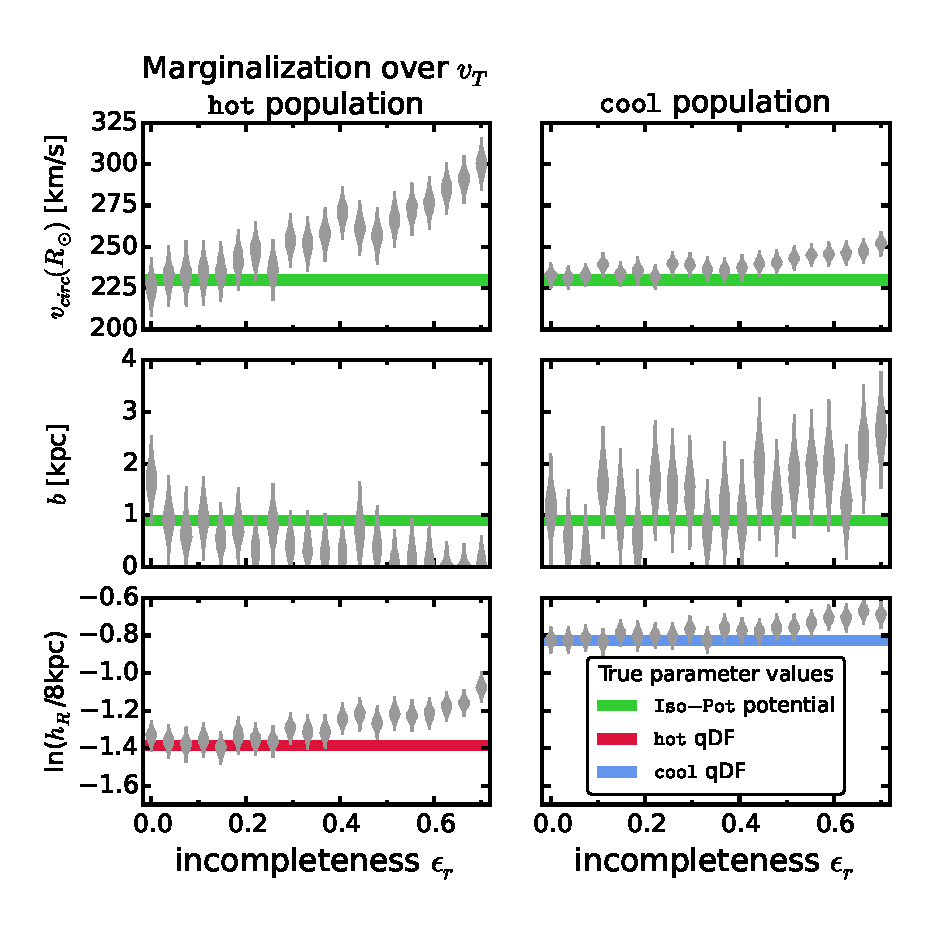
\includegraphics[width=\columnwidth]{figs/isoSphFlexIncompR_marginal_violins_3.eps}
\caption{Same as Figure \ref{fig:isoSphFlexIncompR_violins}, but without including information about the tangential velocities in the analysis. This was done by marginalizing the likelihood in Equation \ref{eq:prob} over $v_T$. The parameter recovery is much worse than in Figure \ref{fig:isoSphFlexIncompR_violins} (as can be seen from comparing the parameter ranges on the $y$-axis). This could indicate that much of the information about the potential is actually stored in the rotation curve, i.e. $v_T(R)$, which is not affected by removing stars from the data set. But even if we do not include $v_T$ we can still recover the potential within the errors, at least for small ($\epsilon_z \lesssim 10\%$).} 
\label{fig:isoSphFlexIncompR_marginal_violins}
\end{figure}

\Wilma{[TO DO: Remove vertical incompleteness from test table]}

\subsection{Measurement uncertainties and their effect on the parameter recovery} \label{sec:results_errors}

Measurement uncertainties in proper motions and distance dominate over uncertainties in position on the sky (RA, Dec) and line-of-sight velocity, which can be more accurately determined.

We first investigate the impact of (perfectly known) proper motion uncertainties on the precision of the potential parameter recovery (see Test \ref{test:isoSphFlexErrConv_SE_vs_error} in Table \ref{tbl:tests}). Figure \ref{fig:isoSphFlexErrConv_SE_vs_error} demonstrates that for data sets with $\delta \mu$ as high as $5~\text{mas yr}^{-1}$ the precision degrades by  a factor of no more than $\sim2$ as compared to a data set without measurement uncertainties. The precision gets monotonically better for smaller $\delta \mu$, being larger only by a factor of $\sim 1.15$ at $\delta \mu=1~\text{mas yr}^{-1}$. With relative standard errors on the recovered parameters of only a few percent at most for 10,000 stars, this means we still get quite precise constraints on the potential, as long as we know the proper motion uncertainties perfectly.

%=============================================================

\begin{figure}[!htbp]
\centering
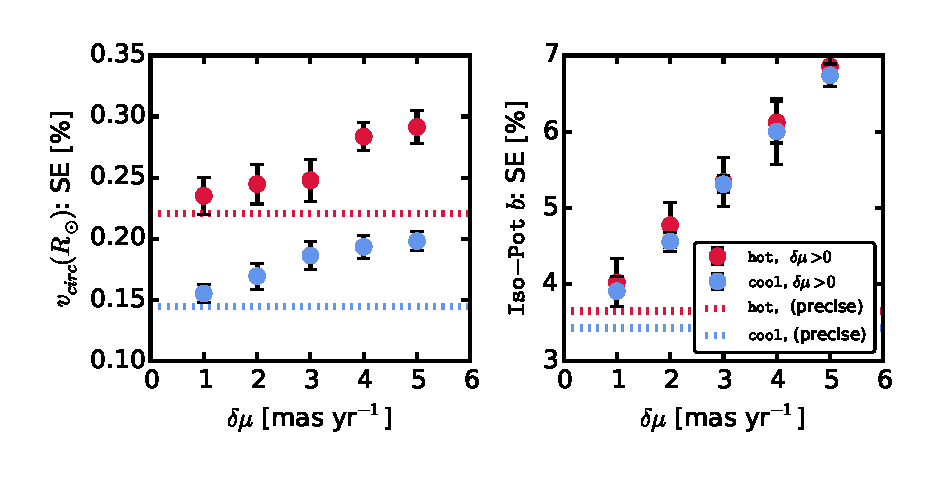
\includegraphics[width=\columnwidth]{figs/isoSphFlexErrConv_SE_vs_error.eps}
\caption{Effect of proper motion uncertainties $\delta \mu$ on precision of potential parameter recovery for two stellar populations of different kinematic temperature (see Test \ref{test:isoSphFlexErrConv_SE_vs_error} in Table \ref{tbl:tests} for all model parameters). The relative standard error (SE) derived from the marginalized \pdf{} for each model parameter was determined for precise data sets without measurement uncertainties (solid lines, with dotted lines indicating the error) and for data sets affected by different proper motion uncertainties $\delta \mu$ and $\delta v_\text{los}=2~\text{km s}^{-1}$ (data points with errors), but no uncertainties in position. The errors come from taking the mean over the results from several data sets.}
\label{fig:isoSphFlexErrConv_SE_vs_error}
\end{figure}


%=============================================================

\begin{figure}[!htbp]
\centering
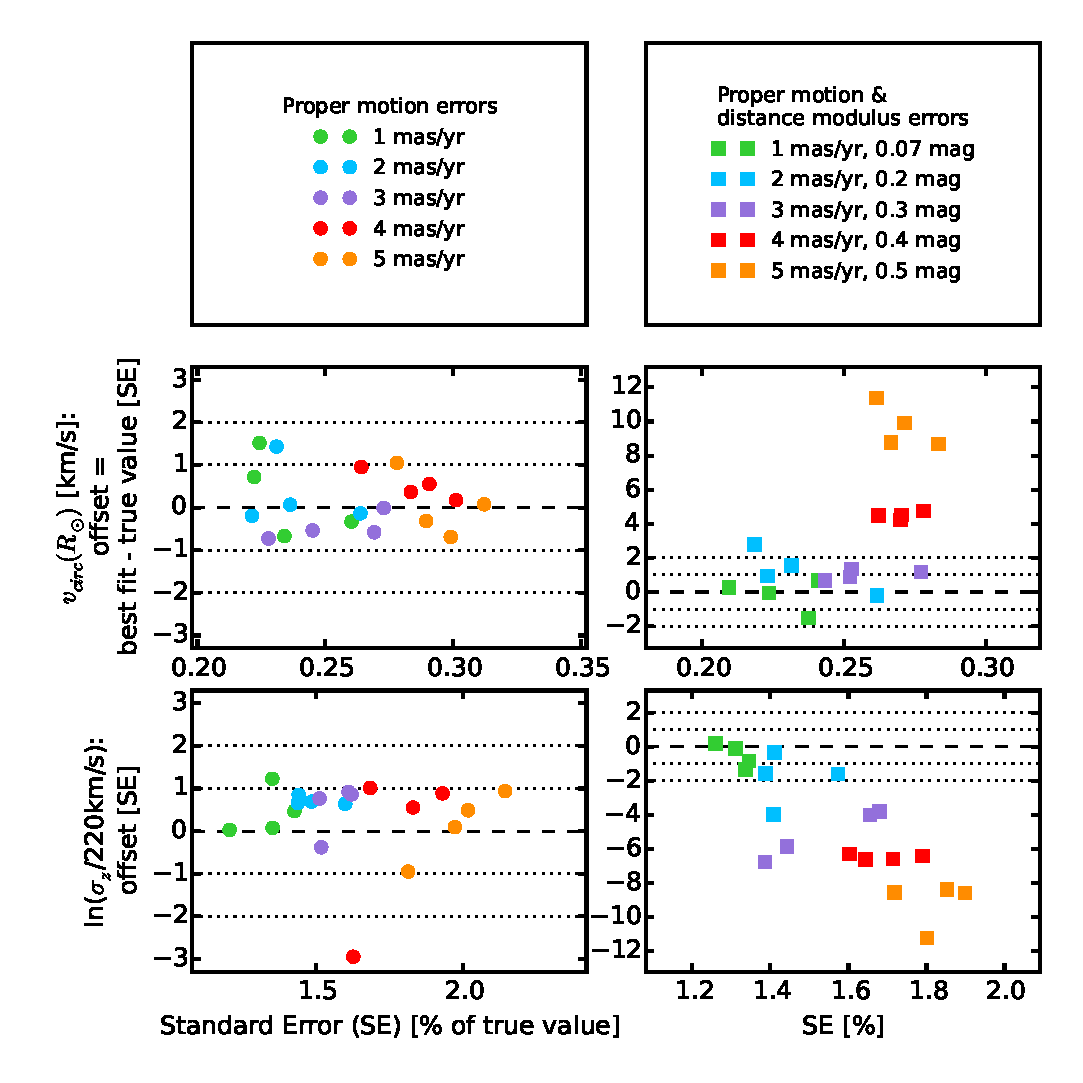
\includegraphics[width=\columnwidth]{figs/isoSphFlexErrConv_bias_vs_SE.eps}
\caption{Potential parameter recovery using the approximation for the model probability convolved with measurement uncertainties in Equation \ref{eq:errorconv}. We show  \pdf{} offset and relative width (i.e., standard error SE) for potential parameters recovered from mock data sets (which were created according to Test \ref{test:isoSphFlexErrConv_bias_vs_SE} in Table \ref{tbl:tests}). The data sets in the left panels are affected only by proper motion uncertainties $\delta \mu$ (and $\delta v_\text{los}=2~\text{mas yr}^{-1}$), while the data sets in the right panels also have distance (modulus) uncertainties $\delta (m-M)$, as indicated in the legend. For data sets with $\delta \mu \leq 3 ~\text{mas yr}^{-1}$ Equation \ref{eq:errorconv} was evaluated with $N_\text{samples}=800$, for $\delta \mu > 3~\text{mas yr}^{-1}$ we used $N_\text{samples}=1200$. In absence of distance uncertainties Equation \ref{eq:errorconv} gives unbiased results. For $\delta(m-M) > 0.2~\text{mag}$ (i.e., $\delta r/r > 0.1$; for $r \lesssim 3~\text{kpc}$) however biases of several sigma are introduced as Equation \ref{eq:errorconv} is only an approximation for the true likelihood in this case.}
\label{fig:isoSphFlexErrConv_bias_vs_SE}
\end{figure}




%=============================================================

\begin{figure}[!htbp]
\centering
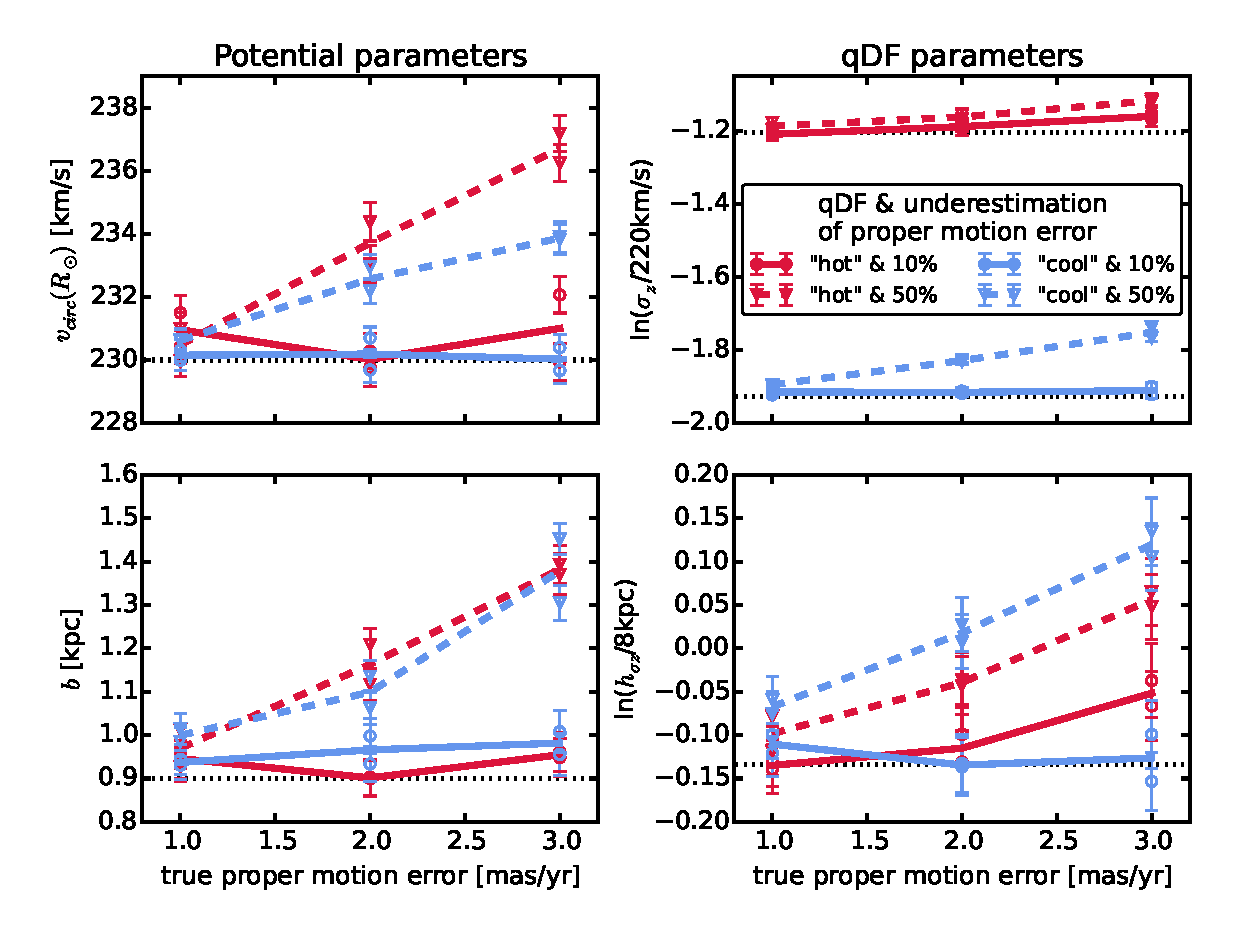
\includegraphics[width=\columnwidth]{figs/isoSphFlexErrSyst_offset_vs_error.eps}
\caption{Effect of a systematic underestimation of proper motion uncertainties $\delta \mu$ in the recovery of the model parameters. (The true model parameters used to create the mock data are summarized as Test \ref{test:isoSphFlexErrSyst} in Table \ref{tbl:tests}, four of them are indicated as black dotted lines in this figure.) The velocities of the mock data were perturbed according to Gaussian uncertainties in the RA and Dec proper motions as indicated on the $x$-axis. The circles and triangles are the best fit parameters of several mock data sets assuming the proper motion uncertainty, with which the model probability was convolved, was underestimated in the analysis by 10\% or 50\%, respectively. The error bars correspond to 1 sigma confidence. The solid lines connect the mean of each two data realisations and are just to guide the eye.}
\label{fig:isoSphFlexErrSyst}
\end{figure}

%=============================================================


We also note that in this case the relative and absolute difference in recovered precision between the precise and the uncertainty-affected data sets does not seem to depend strongly on the kinematic temperature of the stellar population.

Secondly, we investigate the impact of additional measurement uncertainties in distance (modulus). In absence of distance uncertainties the uncertainty-convolved model probability given in Equation \ref{eq:errorconv} is unbiased (see upper left panel in Figure \ref{fig:isoSphFlexErrConv_bias_vs_SE}).  When including distance (modulus) uncertainties, Equation \ref{eq:errorconv} is just an approximation for the true likelihood; the systematic bias thus introduced in the parameter recovery gets larger with the size of $\delta (m-M)$, as demonstrated in Figure \ref{fig:isoSphFlexErrConv_bias_vs_SE}, lower panels (see also Test \ref{test:isoSphFlexErrConv_bias_vs_SE} in Table \ref{tbl:tests}).  We find however that in case of $\delta(m-M) \lesssim 0.2 \text{ mag}$ (if also $\delta \mu \lesssim 2 ~\text{mas yr}^{-1}$ and a maximum distance of $r_\text{max} = 3~\text{kpc}$, see Test \ref{test:isoSphFlexErrConv_bias_vs_SE} in Table \ref{tbl:tests}) the potential parameters can still be recovered within 2 sigma. This corresponds to a relative distance uncertainty of $\sim10\%$. The overall precision of the potential recovery is also not degraded much by introducing distance uncertainties of less than $10\%$.

We therefore found that in case we perfectly knew the measurement uncertainties (and the distance uncertainty is negligible), the convolution of the model probability with the measurement uncertainties gives \emph{precise and accurate} constraints on the model parameters---even if the measurement uncertainty itself is quite large.

Lastly, Figure \ref{fig:isoSphFlexErrSyst} now investigates the effect of a systematic \emph{underestimation} of the true proper motion uncertainties $\delta \mu$ by 10\% and 50\% (see also Test \ref{test:isoSphFlexErrSyst} in Table \ref{tbl:tests}). We find that this causes a bias in the parameter recovery that grows seemingly linear with $\delta \mu$. For an underestimation of only $10\%$ however, the bias is still $\lesssim 2$ sigma for 10,000 stars---even for $\delta \mu \sim 3~\text{mas yr}^{-1}$.

The size of the bias also depends on the kinematic temperature of the stellar population and the model parameter considered (see Figure \ref{fig:isoSphFlexErrSyst}). The qDF parameters are for example better recovered by hotter populations. This is, because the \emph{relative} difference between the true $\sigma_i(R)$ (with $i \in \{R,z\}$) and measured $\sigma_i(R)$ (which comes from the deconvolution with an underestimated velocity uncertainty) is smaller for hotter populations. 

%\subsection{The Impact of Deviations of the Data from the Idealized qDF} \label{sec:results_mixedDFs}

%Motivation of the test and what we're doing
Our modelling approach assumes that each \MAP{} follows a quasi-isothermal distribution function, qDF. In this Section we explore what happens if this idealization does not hold. We investigate this issue by creating mock data sets (Figure \ref{fig:isoSphFlexMix_mockdata_residuals}) that are drawn from two distinct qDFs of different temperature, and analyze the composite mock data set by fitting a single qDF to it. These results are illustrated in Figures \ref{fig:isoSphFlexMixCont} and \ref{fig:isoSphFlexMixDiff}. Following the observational evidence, \MAPs{} with cooler qDFs also have longer tracer scale lengths. In the first set of test, we choose qDFs of widely different temperatures and vary their relative fraction (dubbed \emph{Examples 1a/b} in Figure \ref{fig:isoSphFlexMixCont} and Test \ref{test:isoSphFlexMix} in Table \ref{tbl:tests}); in the second set of tests (\emph{Examples 2a/b} in Figure \ref{fig:isoSphFlexMixDiff} and Test \ref{test:isoSphFlexMix}in Table \ref{tbl:tests}), we always mix mock data points from two different qDFs in equal proportion, but vary by how much the qDF's temperatures differ. 
\\The first set of tests mimics a DF that has wider wings or a sharper core in velocity space than a qDF (Figure \ref{fig:isoSphFlexMix_mockdata_residuals}). The second test could be understood as mixing neighbouring \MAPs{} due to large bin sizes or abundance measurement errors.

%What we see in the plot
It is worth considering the impact of the DF deviations on the recovery of the potential and of the qDF parameters separately. We find from Example 1 that the potential parameters can be better and more robustly recovered, if a mock-data \MAP{} is polluted by a modest fraction ($\lesssim 30\%$) of stars drawn from a much cooler qDF with a longer scale length, as opposed to the same pollution of stars drawn from a hotter qDF with a shorter scale length. 
\\When considering the case of a 50/50 mix of contributions from different qDFs in Example 2, there is a systematic, but only small, error in recovering the potential parameters, monotonically increasing with the qDF parameter difference; in particular for fractional differences in the qDF parameters of $\lesssim 20\%$ the systematics are insignificant even for samples sizes of 20,000, as used in the mock data. 
\\Overall, mock data drawn from a cooler DF always seem to give tighter constraints on the circular velocity at the Sun \Wilma{[TO DO: Make sure that Sun is written everywhere with a capital S.]}, because the rotation curve can be constrained easier if more stars are on near-circular orbits. But we found the recovered $v_\text{circ}(R_\odot)$ not always to be unbiased at the implied precision.
\\The recovery of the effective qDF parameters, in light of non-qDF mock data is quite intuitive: the effective qDF temperature lies between the two temperatures from which the mixed DF of the mock data was drawn; in all cases the scale length of the velocity dispersion fall-off, $h_{\sigma,R}$ and $h_{\sigma,z}$, is shorter, because the stars drawn form the hotter qDF dominate at small radii, while stars from the cooler qDF (with its longer tracer scale length) dominate at large radii. The recovered tracer scale lengths, $h_R$ vary smoothly between the input values of the two qDFs that entered the mix of mock data, with again the impact of contamination by a hotter qDF (with its shorter scale length in this case) being more important. Overall, we find that the potential inference is quite robust to modest deviations of the data from the assumed DF.



%====================================================================

%FIGURE: isoSphFlexMix_mockdata_residuals

\begin{figure*}[!htbp]
\plotone{figs/isoSphFlexMix_mockdata_residuals.eps}
\caption{Distribution of mock data, created by mixing stars drawn from two different qDFs (solid lines), and the distribution predicted by the best fit of a single qDF and potential to the data (dashed lines). The model parameters to create the mock data (solid lines) are given in Table \ref{tbl:tests} as Test \ref{test:isoSphFlexMix}, and the qDF parameters referenced in the figure's legend are given in Table \ref{tbl:referenceMAPs}. The corresponding single qDF best-fit curves (dashed lines) were created by drawing mock data from the best fit parameters found in Figures \ref{fig:isoSphFlexMixCont} and \ref{fig:isoSphFlexMixDiff}. \emph{Example 1:} Distribution of mock data drawn from a superposition of two very different (but fixed) qDFs at varying mixing rates. \emph{Example 2:} Mock data distribution of two \MAPs{} that were mixed at a fixed rate of 50\%/50\%, but the difference of the qDF parameters of one \MAP{} was varied with respect to the qDF parameters of the other \MAP{} by $X\%$ (see Table \ref{tbl:referenceMAPs}). The data sets are color coded in the same way as the corresponding analyses in Figures  \ref{fig:isoSphFlexMixCont} and \ref{fig:isoSphFlexMixDiff}. This figure demonstrates how mixing two qDFs can be used as a test case for changing the shape of the DF to not follow a pure qDF anymore, e.g. by adding wings or slightly changing the radial density profile. When comparing the mock data and best fit distribution, we see that especially for the most extreme deviations it becomes obvious that a single qDF is a bad assumption for the stars' \emph{true} DF. \Wilma{[TO DO: Potential and/or population names in typewriter font] [TO DO: include $X$ somehow in figure to explain it better. Jo didn't understand what I meant by it in this caption.] [TO DO: These are really many panels. Try to remove some.]}}
\label{fig:isoSphFlexMix_mockdata_residuals}
\end{figure*}


%FIGURE: isoSphFlexMixCont

\begin{figure*}[!htbp]
\centering
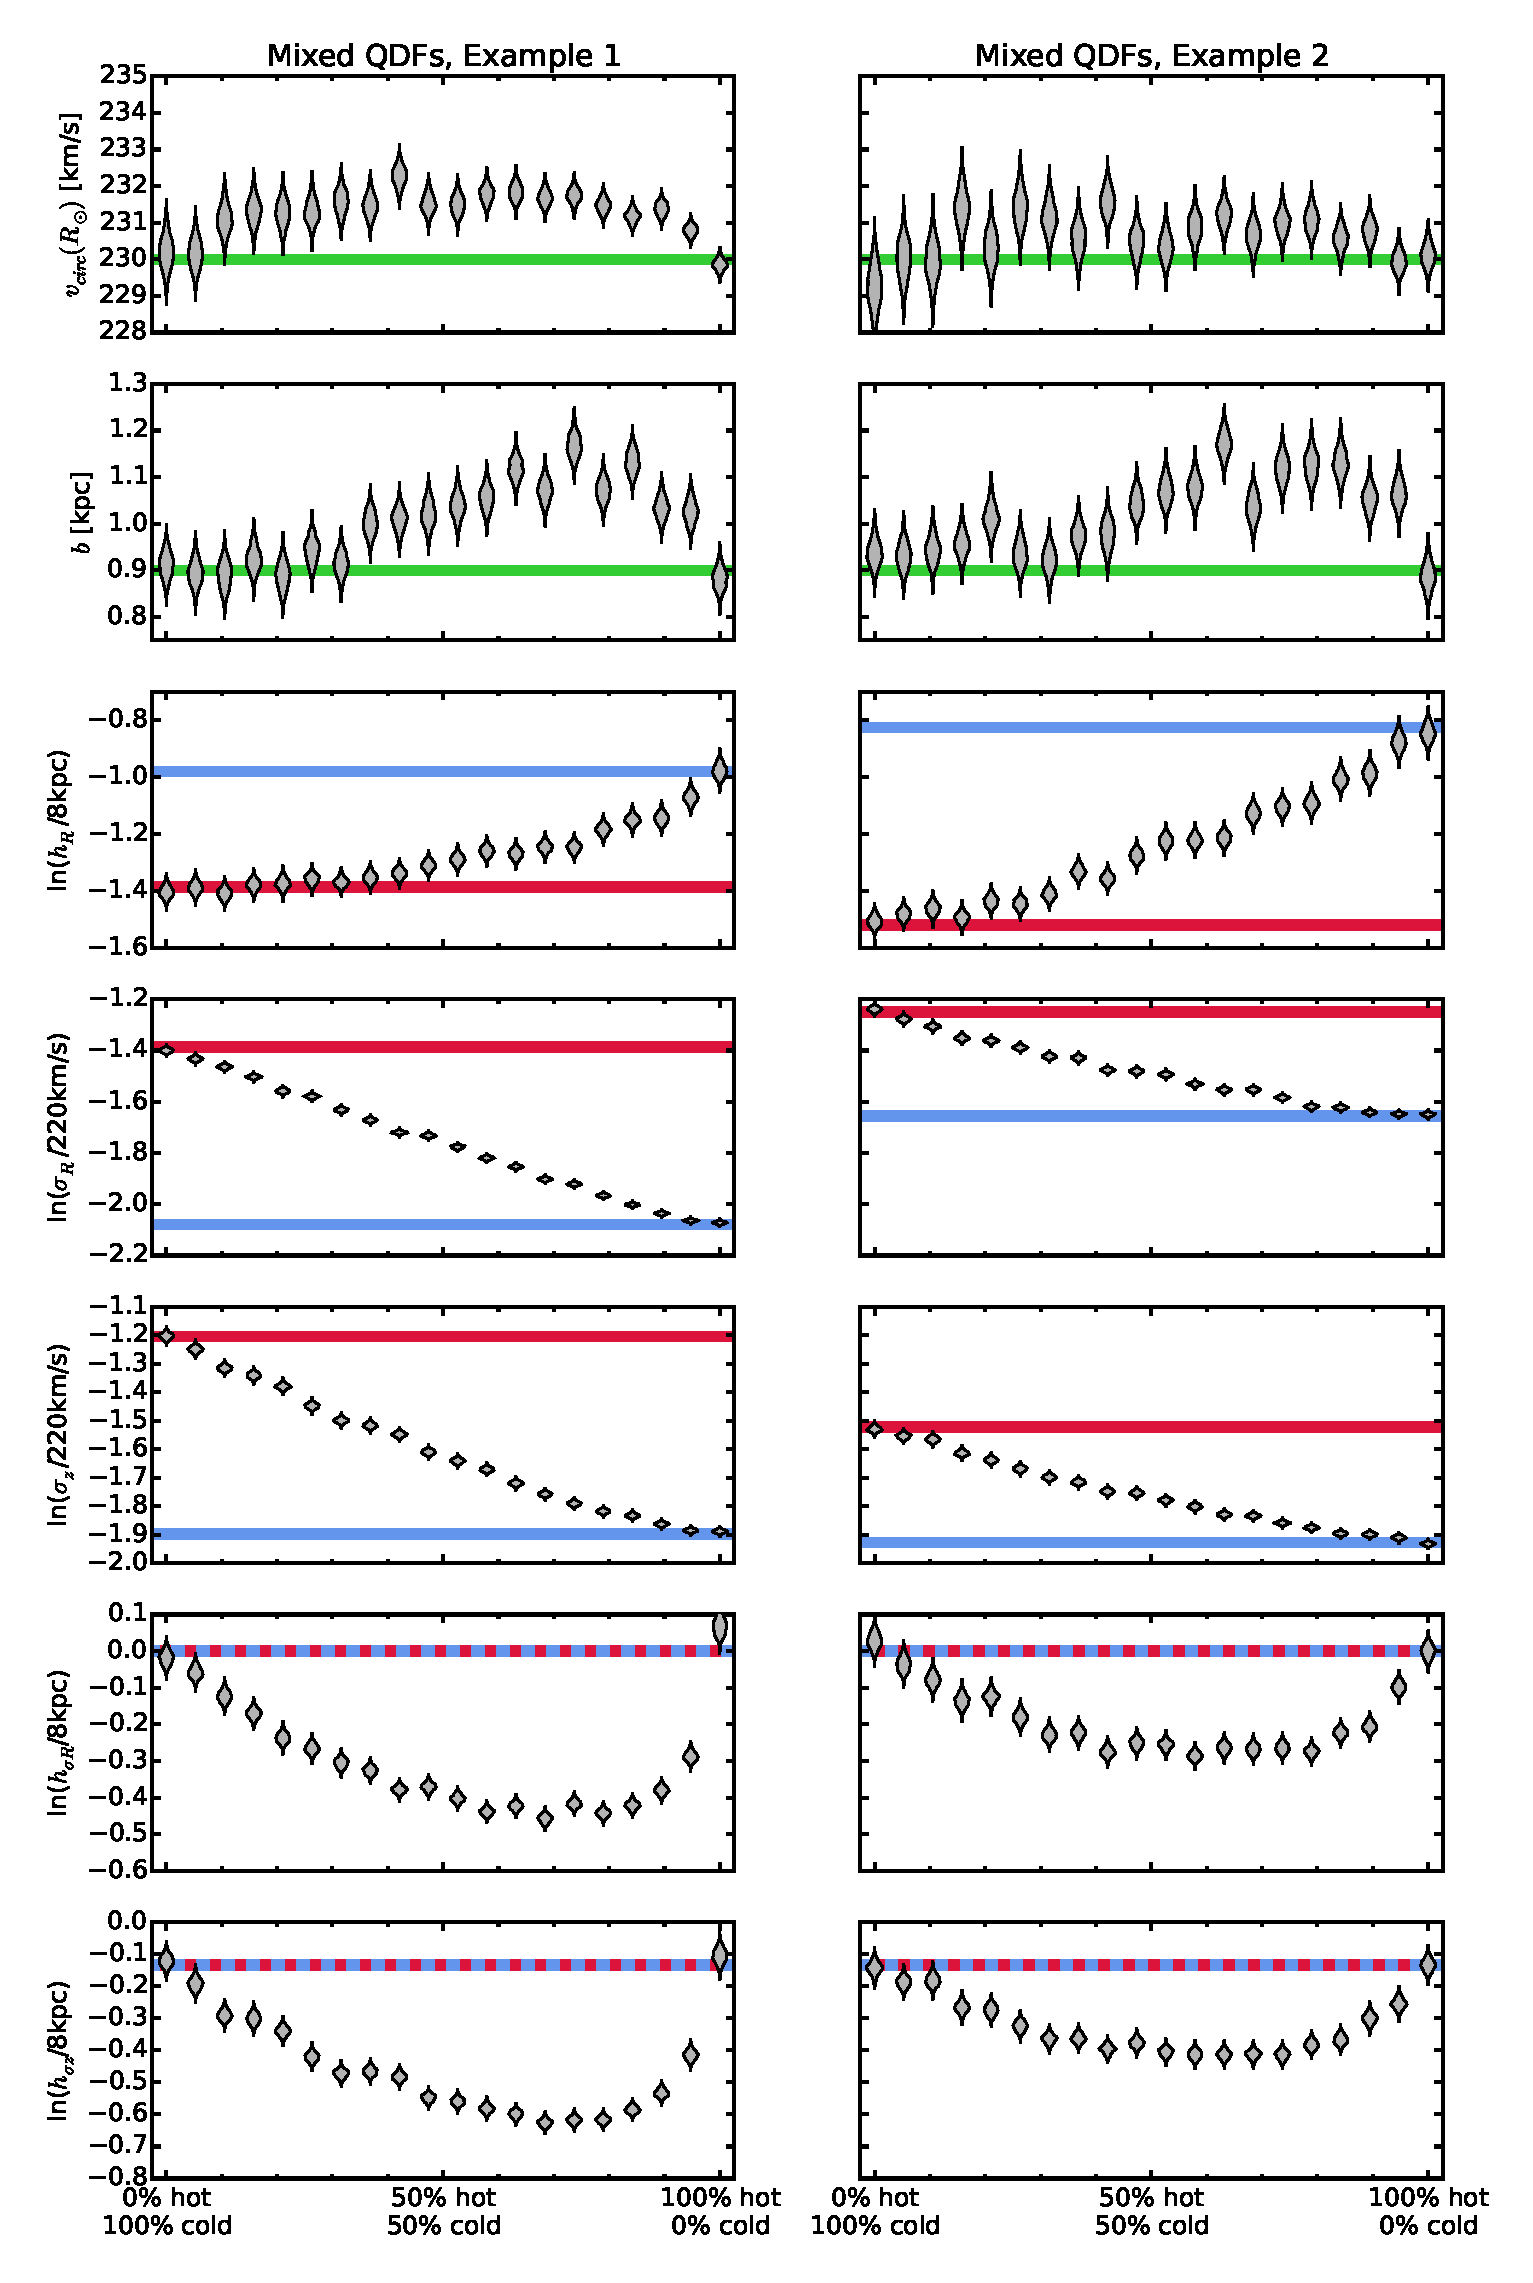
\includegraphics[width=0.8\textwidth]{figs/isoSphFlexMixCont_violins.eps}
\caption{The dependence of the parameter recovery on degree of pollution and temperature of the stellar population. To model the pollution of a hot stellar population by stars coming from a cool population and vice versa, we mix varying amounts of stars from two very different populations, as indicated on the $X$-axis. The composite mock data set is then fit with one single qDF. The violins represent the marginalized likelihoods found from the MCMC analysis. \emph{Example 1a} (\emph{Example 1b}) in the left (right) panels mixes the \texttt{hot} (\texttt{cool}) \MAP{} with the \texttt{cooler} (\texttt{hotter}) \MAP{} in Table \ref{tbl:referenceMAPs}. All model parameters used to create the mock data are given in Test \ref{test:isoSphFlexMix}, \emph{Example 1a) \& b)} in Table \ref{tbl:tests}. Some mock data sets are shown in Figure \ref{fig:isoSphFlexMix_mockdata_residuals}, first two rows, in the same colors as the violins here.  We find that a hot population is much less affected by pollution with stars from a cooler population than vice versa. \Wilma{[TO DO: rename $h_{\sigma R}$ to $h_{\sigma,R}$, $\sigma_R$ to $\sigma_{R,0}$ and analogous for $z$] [TO DO: Potential and/or population names in typewriter font] [TO DO: Comment from Jo: I feel like just showing one of these examples might be clearer, because they essentially demonstrate the same thing.] [TO DO: Remove $\sigma_R$ and $h_{\sigma,R}$ panels. Then make two columns with only one expample, potential and DF parameters separately]}}
\label{fig:isoSphFlexMixCont}
\end{figure*}



%FIGURE: isoSphFlexMixDiff

\begin{figure*}[!htbp]
\centering
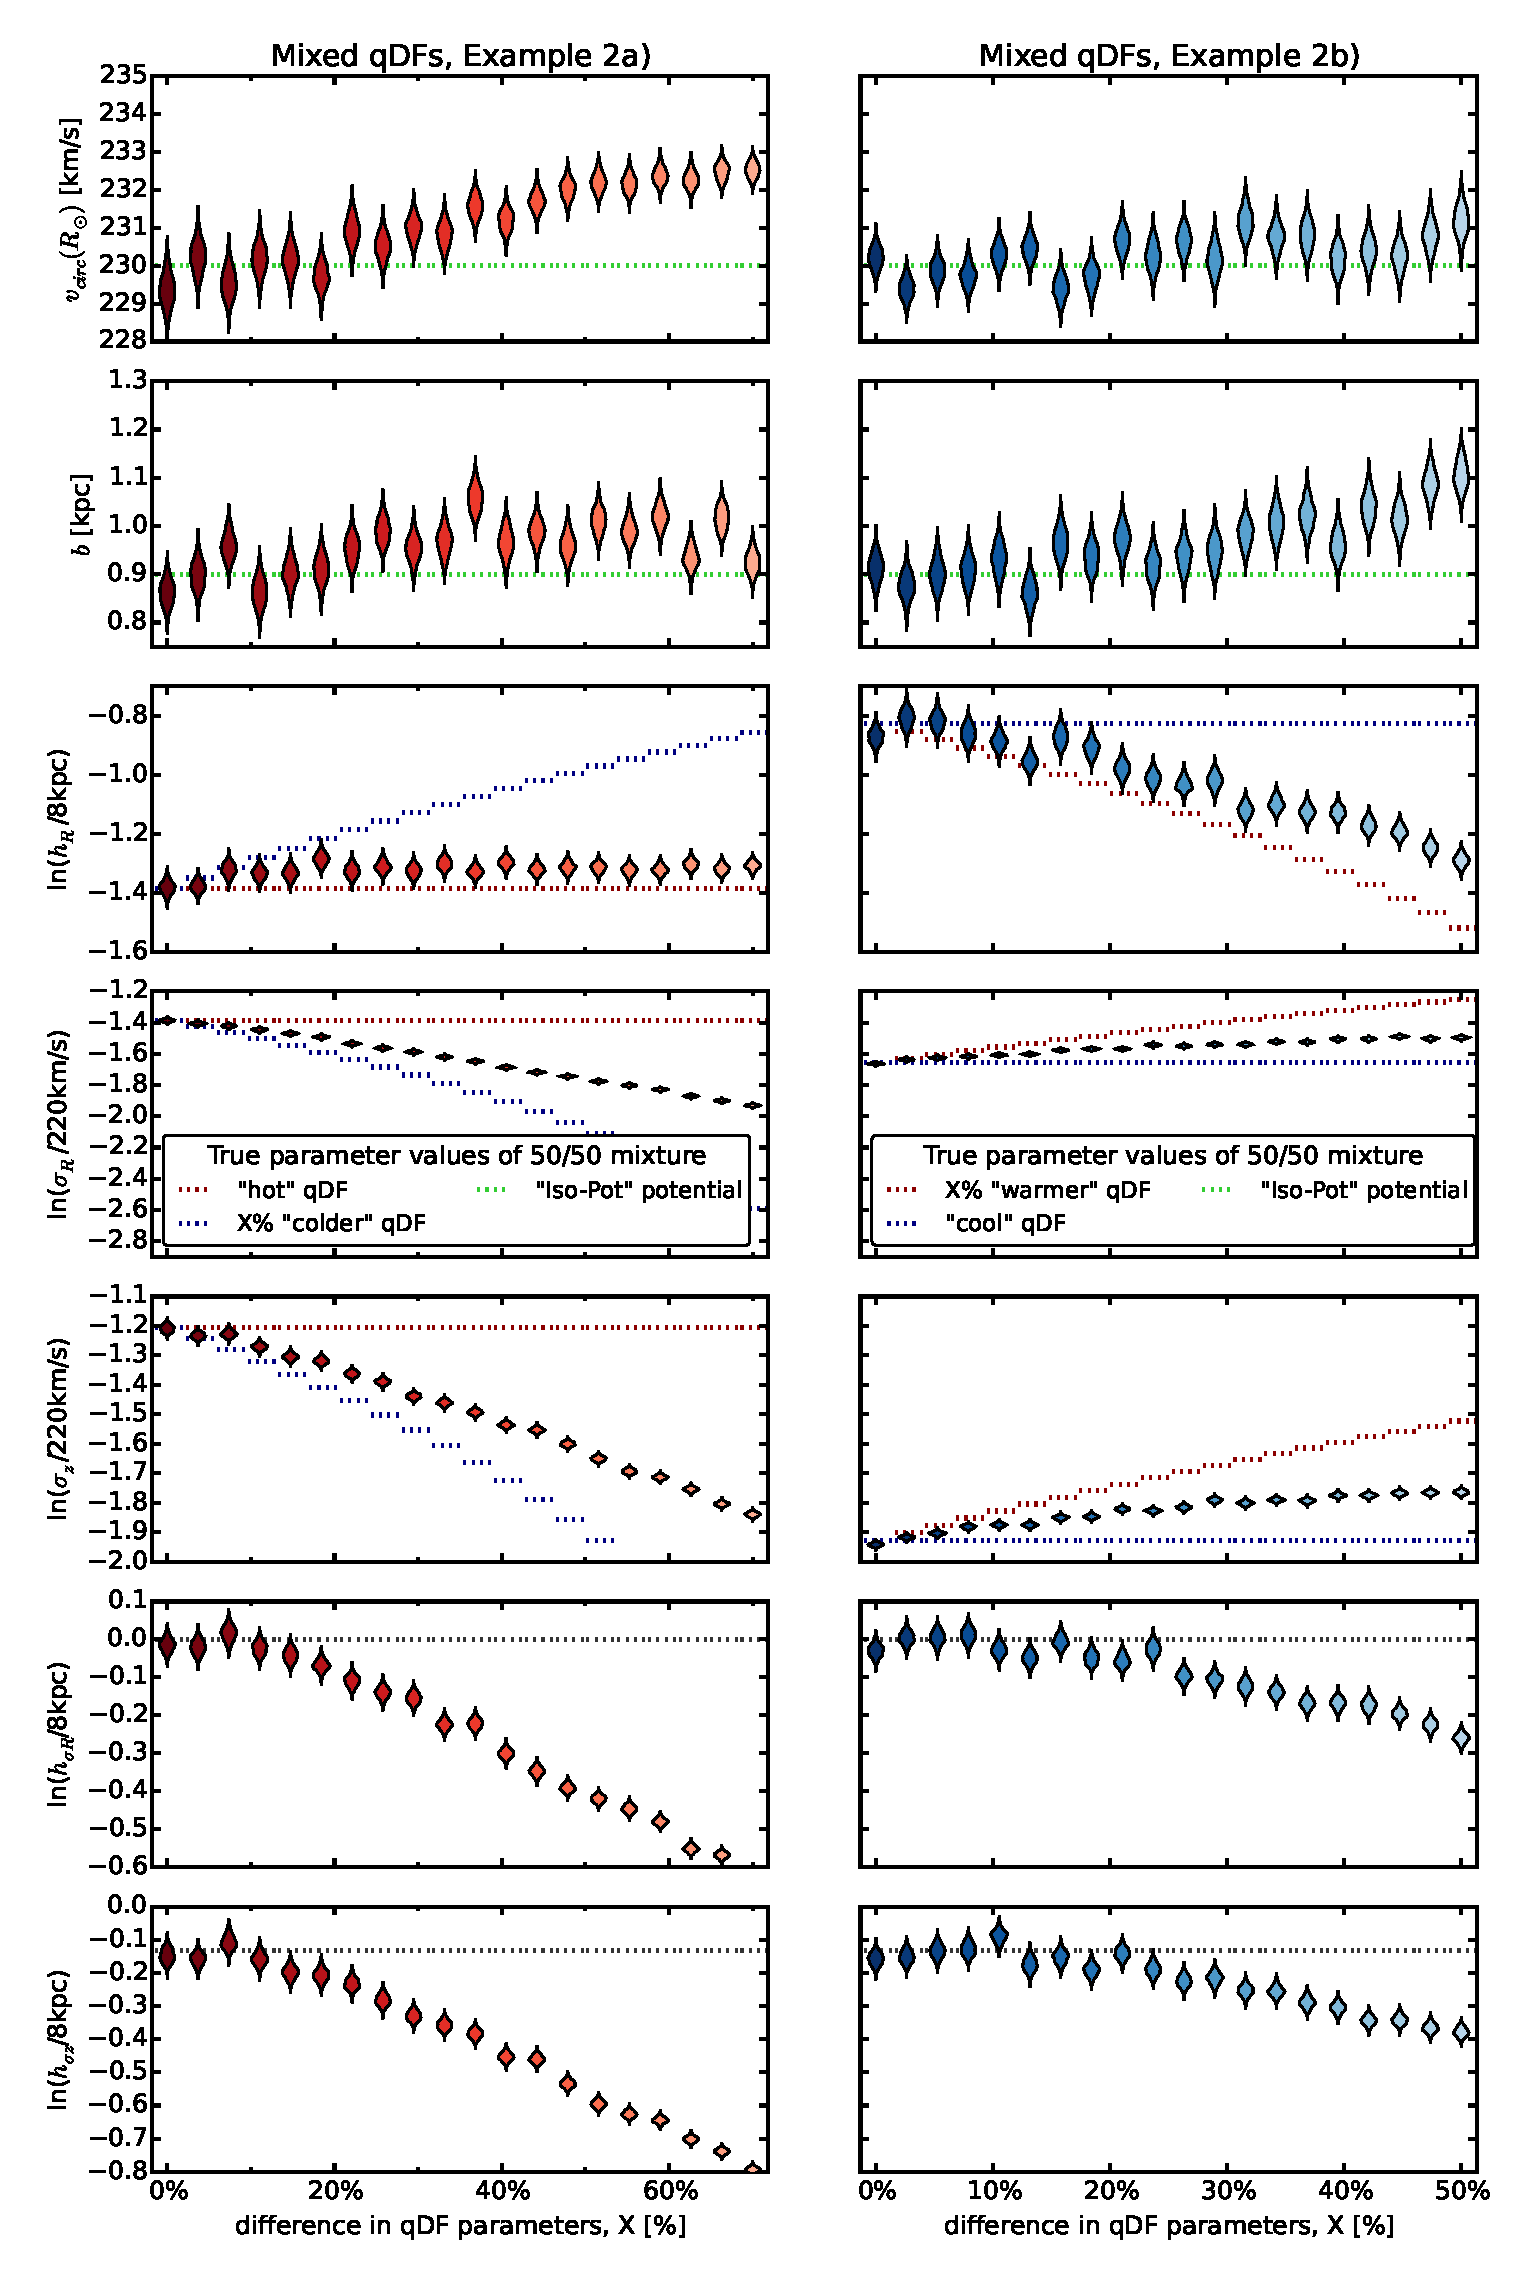
\includegraphics[width=0.8\textwidth]{figs/isoSphFlexMixDiff_violins.eps}
\caption{The dependence of the parameter recovery on the difference in qDF parameters of a 50\%/50\% mixture of two stellar populations and their temperature. Half of the star in each mock data set in \emph{Example 2a} (\emph{Example 2b}) was drawn from the \texttt{hot} (\texttt{cool}) qDF in Table \ref{tbl:referenceMAPs}, and the other half drawn from a \texttt{colder} (\texttt{warmer}) population that has $X\%$ smaller (larger) $\sigma_{R,0}$ and $\sigma_{z,0}$ and $X\%$ larger (smaller) $h_R$. Each composite mock data set is then fitted by a single qDF and the marginalized MCMC likelihoods for the best fit parameters are shown as violins. The model parameters used for the mock data creation are given as Test \ref{test:isoSphFlexMix}, \emph{Example 2a) \& b)} in Table \ref{tbl:tests}. Some mock data sets are shown in figure \ref{fig:isoSphFlexMix_mockdata_residuals}, last two rows, where the distributions have the same colors as the corresponding best fit violins here. By mixing \MAPs{} with varying difference in their qDF parameters, we model the effect of bin size in the [Fe/H]-[$\alpha$/Fe] plane when sorting stars into different \MAPs{}: The smaller the bin size, the smaller the difference in qDF parameters of stars in the same bin. We find that the bin sizes should be chosen such that the difference in qDF parameters between neighbouring \MAPs{} is less than 20\%. \Wilma{[TO DO: rename $h_{\sigma R}$ to $h_{\sigma,R}$, $\sigma_R$ to $\sigma_{R,0}$ and analogous for $z$] [TO DO: Potential and/or population names in typewriter font]}} 
\label{fig:isoSphFlexMixDiff}
\end{figure*}

%====================================================================

%\subsection{The Implications of a Gravitational Potential not from the Space of Model Potentials} \label{sec:results_potential}

%Motivation for the Test

We now explore what happens when the mock data were drawn from one axisymmetric potential family, here \texttt{MW14-Pot}, and is then modelled considering potentials from only another axisymmetric family, here \texttt{KKS-Pot} (compare the second and fourth panel in Figure \ref{fig:ref_pots}). In the analysis we assume the circular velocity at the Sun to be fixed and known \Wilma{[TO DO: Comment from Hans-Walter: Do we have reason to believe that this very restrictive assumption does not qualitatively impact our upshot (quantitative differences are OK).]} and only fit the parametric potential form. The results are shown in Figure \ref{fig:MW14vsKKS2SphFlex}.




%Results on the potential

The reference potential parameters \HW{[TO DO: Comment from HW: What does "reference" mean here exactly? Is this an independent exercise, to ask which parameters are expected when fitting potential to potential? (I don't know, what he means...)]} of the \texttt{KKS-Pot} in Table \ref{tbl:referencepotentials} were found by adjusting the 2-component Kuzmin-Kutuzov St\"{a}ckel potential by \citet{1994AA...287...43B} such that it generates radial and vertical force profiles similar to the \texttt{MW14-Pot} from \citet{2015ApJS..216...29B} (dotted gray lines in Figure \ref{fig:MW14vsKKS2SphFlex}). We then run \RM{} using these ``inconsistent'' families of gravitational potentials, and find a good fit to the data in configuration space (see Figure \ref{fig:MW14vsKKS2SphFlex_mockdata_residuals}). The results from \RM{} analysis for the potential shown in Figure \ref{fig:MW14vsKKS2SphFlex}, red for a \texttt{hot} mock data \MAP{} and blue for a \texttt{cool} \MAP{}, give an comparable good or even better agreement with the true potential than the (by-eye) fit directly to the potential: especially the force contours, to which the orbits are sensitive, and the rotation curve are very tightly constrained and reproduce the true potential even outside of the observed volume of the mock tracers. This demonstrates that \RM{} fitting inferres a potential that in its actual properties resembles the input potential for the mock data as closely as possible, given the differences in functional forms.
\\The density contours are less tightly constrained than the forces, but we still capture the essentials: the \texttt{hot} \MAP{} from Table \ref{tbl:referenceMAPs} constrains the halo; especially at smaller radii it is equally good or better than the \texttt{cool} \MAP{}. The \texttt{cool} \MAP{} gives tighter constraints on the halo in the outer region and recovers the disk better than the \texttt{hot} \MAP{}. This is in concordance with expectations as the \texttt{cool} \MAP{} has a longer tracer scale length and is more confined to the disk than the \texttt{hot} \MAP{} and therefore also probes the Galaxy in these regions better.
\\Overall the best fit disk is less dense in the midplane than the true disk. 

%Results on the qDF

Figure \ref{fig:MW14vsKKS2SphFlex_violins} compares the true qDF parameters with the best fit parameters for this case. While tracer scale length and radial velocity dispersion profile are very well recovered, we misjudge the radial profile of the vertical velocity dispersion as $\sigma_{0,z}$ and $h_{\sigma,z}$ are both underestimated, which leads to a steeper profile and a lower dispersion around the Sun.






%====================================================================

\begin{figure*}
\plotone{figs/MW14vsKKS2SphFlex_mockdata_residuals.eps}
\caption{Comparison of the distribution of mock data in configuration space created in the \texttt{MW14-Pot} potential (solid lines) with a \texttt{hot} (red) and \texttt{cool} (blue) \MAP{} (Test \ref{test:MW14vsKKS2SphFlex} in Table \ref{tbl:tests}), and the best fit distribution using a \texttt{KKS-Pot} potential (dashed lines). The best fit potentials are shown in Figure \ref{fig:MW14vsKKS2SphFlex} and the corresponding best fit qDF parameters in Figure \ref{fig:MW14vsKKS2SphFlex_violins}. The best fit \Wilma{[TO DO: Continue Caption, Jo suggests add something about the fit being good.] [TO DO: Potential and/or population names in typewriter font]}}
\label{fig:MW14vsKKS2SphFlex_mockdata_residuals}
\end{figure*}


\begin{figure*}
\plotone{figs/MW14vsKKS2SphFlex_contours_compare.eps}
\caption{Recovery of the gravitational potential if the assumed potential model (\texttt{KKS-Pot} with fixed $v_\text{circ}(R_\odot)$) and the true potential of the (mock) stars (\texttt{MW14-Pot} in Table \ref{tbl:referencepotentials}) is slightly different. We show the circular velocity curve, as well as contours of equal density, radial and vertical force in the $R$-$z$-plane, and compare the true potential with 50 \Wilma{[TO DO: CHECK]} sample potentials drawn from the posterior distribution function found with the MCMC for a \texttt{hot} (red) and a \texttt{cool} \MAP{} (blue). All model parameters are given as Test \ref{test:MW14vsKKS2SphFlex} in Table \ref{tbl:tests}. \Wilma{[TO DO: Do more analyses???] [TO DO: fancybox Legend] [TO DO: Potential and/or population names in typewriter font] [TO DO: Reference correct Table in Plot - don't forget!] [TO DO: Redo whole analysis with vcirc not being fixed (HW is not sure if this really doesn't make a difference.]} \Wilma{[TO DO: Comment from Jo: Maybe better with twice as many contour levels? Now not that many within the yellow curve.]}}
\label{fig:MW14vsKKS2SphFlex}
\end{figure*}

\begin{figure*}
\plotone{figs/MW14vsKKS2SphFlex_violins.eps}
\caption{Recovery of the qDF parameters for the case where the true and assumed potential deviate from each other (Test \ref{test:MW14vsKKS2SphFlex} in Table \ref{tbl:tests}). The thick red (blue) lines represent the true qDF parameters of the \texttt{hot} (\texttt{cool}) qDF in Table \ref{tbl:referenceMAPs} used to create the mock data, surrounded by a 10\% error region. The grey violins are the marginalized likelihoods for the qDF parameters found simultaneously with the potential constraints shown in Figure \ref{fig:MW14vsKKS2SphFlex}. \Wilma{[TO DO: rename $h_{\sigma R}$ to $h_{\sigma,R}$, $\sigma_R$ to $\sigma_{R,0}$ and analogous for $z$]}}
\label{fig:MW14vsKKS2SphFlex_violins}
\end{figure*}


%====================================================================





%%-----------------------------------------------------------------------------------------------------------------------------------------------------------------------------
%
%%-----------------------------------------------------------------------------------------------------------------------------------------------------------------------------
%%Discussion etc.
\section{Discussion and Summary} \label{sec:discussionsummary}

\Wilma{[TO DO: Introduce DF somewhere - use DF wherever we don't need qDF.] [TO DO: Introduce MW somewhere.]}
\\\Wilma{[TO DO: Compare these sections with the results. Points should be made detailed in the results section and short here in the discussion. Says Hans-Walter.]}
\\\Wilma{[TO DO: Absätze mit Indent. Keine Leerzeilen.]}

%Setting the Context
Recently, implementations of action DF-based modelling of 6D data in the Galactic disk have been put forth, in part to lay the ground-work fo Gaia (BR13; \citealt{,2013MNRAS.433.1411M,2014MNRAS.445.3133P,2015MNRAS.449.3479S}).

%Everything in a nutshell
We present \RM{}, an improved implementation of the dynamical modelling machinery of BR13, to recover the MW's gravitational potential by fitting an orbit distribution function to stellar populations within the Galactic disk. In this work we investigated the capabilities, strengths and weaknesses of \RM{} by testing its robustness against the breakdown of some of its assumptions---for well-defined, isolated test cases using mock data. Overall the method works very well and is reliable, even when there are small deviations of the model assumptions from the real world Galaxy.

%The RM code
\RM{} applies a full likelihood analysis and is statistically well-behaved. It goes beyond BR13 by allowing for a straightforward and flexible implementation of different model families for potential and DF. It also accounts for selection effects by using full 3D selection functions (given some symmetries).\\

\noindent {\bf Computational speed:~} Large data sets in the age of Gaia require increasingly accurate likelihood evaluations and flexible models. To be able to deal with these computational demands, we sped up the \RM{} code by combining a nested grid approach with MCMC and by faster action calculation using the St\"{a}ckel \citep{2012MNRAS.426.1324B} interpolation grid by \citet{2015ApJS..216...29B}. However, application of \RM{} to millions of stars will still be a task for supercomputers and calls for even more improvements and speed-up in the fitting machinery.\\

\noindent {\bf Properties of the data set:~} We could show that \RM{} can provide potential and DF parameter estimates that are very accurate (i.e. unbiased) and precise in the the limit of large datasets, as long as the modelling assumptions are fulfilled. We also found that the \emph{location} of the survey volume within the Galaxy matters little. At given sample size a larger survey \emph{volume} with large coverage in \emph{both radial and vertical} direction will give the tightest constraints on the model parameters. \Wilma{[TO DO: Finished up to here. Continue here.]}
\\Stellar populations of different scale length and temperature probe different regions of the Galaxy (BR13). But there is no easy rule of thumb for which survey volume and stellar population which potential and DF parameter is constrained best.\\
Surprisingly, (cf. \citealt{2013A&ARv..21...61R}) \RM{} seems to be very robust against misjudgments in the selection function of the data. We speculate that this is because missing stars in the data set do not affect the connection between a star's velocity and position, which is given by the potential. Much of the information about the potential profile is stored in the rotation curve, but we find that even when when we do not include measurements of tangential velocities in the analysis, small misjudgments of the incompleteness do not affect the potential recovery.\\

\Wilma{[TO DO: Comment from HW: Author: rix Subject: This paragraph shouldbe 1 or 2 sentences, following the first paragraph on "Sample/Data Properties". This -- at the moments --reads to bequite confusing. I don't quite get whatthe "upshot" is; there is technical detai on $N_{error}$ [enought to say it's expensive]; and, as noted earlier; I don't understand why theerror convolution for a nearbydata point needs to know about $\delta v_\text{max}$]} Properly convolving the likelihood with measurement errors is computational very expensive. By ignoring positional errors and only including distance errors as part of the velocity error, we can drastically reduce the computational costs. For stars within 3 kpc from the sun this approximation works well for distance errors of $\sim 10\%$ or smaller. The number of MC samples needed for the error convolution using MC integration scales by $N_\text{error} \propto (\delta v_\text{max})^2$ with the maximum velocity error at the edge of the sample. If we did not know the true size of the proper motion measurement errors perfectly, we can only reproduce the true model parameters to within $\lesssim 2$ sigma \Wilma{[TO DO: Check???]} as long as we do not underestimate it by more than $10\%$ and for proper motion errors $\lesssim 2 \text{ mas yr}^{-1}$.\\

%%\subsection{Data Deviations from the Modelling Assumptions about the Distribution Function and the Potential}
%
%\noindent {\bf Deviations from the qDF Assumption:~}  Our modelling is founded on the assumption, that we can identify {\sl a priori} sub-components of the Galactic disk that follow a qDF (e.g., by considering \MAPs{}). There are two reasons why any chosen sub-sample of stars (here a \MAP{}) may not be well described by any qDF. Either, because nature is more complex, or because even if perfect
%\MAPs{} would be well described by qDFs finite abundance errors would mix \MAPs{}.  We have considered both cases. \Wilma{[TO DO: Comment from HW: it feels to me that this is the 3rd time you said this.It's OK to say, but in1 line at most.]}
%\\In Example 1 in \S\ref{sec:results_mixedDFs} we investigated how well we can recover the potential, if this assumption was not perfectly satisfied, i.e., the \MAP{}'s true DF does not perfectly follow a qDF. We considered two cases: a) a hot DF, that has less stars at small radii and more stars with low velocities than predicted by the qDF (reddish data sets in Figure \ref{fig:isoSphFlexMix_mockdata_residuals}), or b) a cool DF that has broader velocity dispersion wings and less stars at large radii than predicted by the qDF (bluish data sets). We find that case a) would give more reliable results for the potential parameter recovery, but in both cases biases are small if the contamination is less than \Wilma{[TO DO: CHECK]}.
%\\If we assumed that the distribution of stars from one \MAP{} is caused by radial migration away from the initial location of star formation, it would more likely that the qDF overestimates the true number of stars at smaller radii than underestimating it at larger radii. \HW{[TO DO: Is this actually a sensible argument??? Jo is not convinced that this is right.]}
%\\Following this, focusing the analysis especially on hotter \MAPs{} could be an advisable way to go in the future, if there is doubt that the stars truly follow the qDF.
%\\Another critical point is the binning of stars into \MAPs{} depending on their metallicity and $\alpha$ abundances. Example 2 in \S\ref{sec:results_mixedDFs} could be understood as a model scenario for decreasing bin sizes in the metallicity-$\alpha$ plane when sorting stars in different \MAPs{}, assuming that there is a smooth variation of qDF within the metallicity-$\alpha$ plane and each \MAP{} indeed follows a qDF. We find that, in the case of 20,000 stars in each bin, differences of $20\%$ in the qDF parameters of two neighbouring bins can still give quite good constraints on the potential parameters. 
%\\We compare this with the relative difference in the qDF parameters in the bins in Figure 6 of BR13, which have sizes of $[\mathrm{Fe}/\mathrm{H}] = 0.1$ dex and $\Delta [\alpha/\mathrm{Fe}] = 0.05$ dex. It seems that these bin sizes are large enough to make sure that $\sigma_{R,0}$ and $\sigma_{z,0}$ of neighbouring \MAPs{} do not differ more than $20\%$. Figure \ref{fig:isoSphFlexMixCont} and \ref{fig:isoSphFlexMixDiff} suggest that especially the tracer scale length $h_R$ needs to be recovered to get the potential right. For this parameter however the bin sizes in Figure 6 of BR13 might not yet be small enough to ensure no more than $20\%$ of difference in neighbouring $h_R$. This is especially the case in the low-$\alpha$ ($[\alpha/\mathrm{Fe}] \lesssim 0.2$), intermediate-metallicity ($[\mathrm{Fe}/\mathrm{H}] \sim -0.5$) \MAPs{}, which where however not used in the dynamical modelling by BR13. The above is valid for 20,000 stars per \MAP{}. In case there are less than 20,000 stars in each bin the constraints are less tight and due to Poisson noise one could also allow larger differences in neighbouring \MAPs{} while still getting reliable results.\\
%\Wilma{[TO DO: Include the following comments by Jo somewhere: This is a general approach of fitting action-based disk DFs for getting the potential. The qDF is a specific example that we use in this paper. In futures studies different forms of DFs might be fitted to data.  That the results are quite robust to the form of the DF not entirely correct motivates this further.]}
%
%\noindent {\bf Gravitational Potential beyond the Parameterized Functions Considered:~} \Wilma{[TO DO: Comment from HW: In style and contentthis seems verysimilar tothe RESULTSsection. We should eitherdrastically shorten the text in the results section (probably not), or here.]} In the long run \RM{} should incorporate a family of gravitational potential models that can reproduce the essential features of the MW's true mass distribution. While our fundamental assumption of the Galaxy's axisymmetry is at odds with the obvious existence of non-axisymmetries in the MW, we will not dive into investigating this implications in this paper. Instead we test how a misjudgment of the parametric potential form affects the recovery by fitting a potential of St\"{a}ckel form \citep{1994AA...287...43B} to mock data from a different potential family with halo, bulge and exponential disk. The recovery is quite successful and we get the best fit within the limits of the model. However, even a strongly flattened St\"{a}ckel potential component has difficulties to recover the very flattened mass distribution of an exponential disk. This leads to misjudgment of the qDF parameters describing the vertical action distribution, $\sigma_{z,0}$ and $h_{\sigma,z}$. As the qDF parameter $\sigma_{z,0}$ corresponds to the physical vertical velocity dispersion at the sun, a comparison with direct measurements could be a valuable cross-checking reference. \Wilma{[TO DO: This might not be true. For isochrone and Staeckel potential I get this behaviour, but not for the MW14-Pot!!! Might be, because it's not separable??? Check!!!] [TO DO: best to simply remove it...]} In case of as many as 20,000 stars we should therefore already be able to distinguish between different potential models.
%\\The advantage of using a St\"{a}ckel potential with \RM{} is firstly the exact and fast action calculation via the numerical evaluation of a single integral, and secondly that the potential has a simple analytic form, which greatly speeds up calculations of forces and frequencies (as compared to potentials in which only the density has an easy description like the exponential disk). A superposition of several simple Kuzmin-Kutuzov St\"{a}ckel components can successfully produce MW-like rotation curves (see \citet{1994AA...287...43B}, \citet{2003MNRAS.340..752F} and Figure \ref{fig:MW14vsKKS2SphFlex}) and one could think of adding even more components for more flexibility, for example a small roundish component for the bulge. \Wilma{[TO DO: Comment by Jo: In a sense the two approaches (a) using the Staeckel action approximation with a MW like potential and (b) using a Staeckel potential directly are dong the same thing (approximating the true potential as a Staeckel potential). The question is which is best.]}
%\\The potential model used by BR13 had only two free parameters (disk scale lentgh and halo contribution to $v_\text{circ}(R_\odot)$. To circumvent the obvious disadvantage of this being at all not flexible enough, they fitted the potential separately for each \MAP{} and recovered the mass distribution for each \MAP{} only at that radius for which it was best constrained - assuming that \MAPs{} of different scale length would probe different regions of the Galaxy best. Based on our results in Figure \ref{fig:MW14vsKKS2SphFlex} this seems to be indeed a sensible approach \Jo{[TO DO: Check that this is indeed the case - it is not clear to me from the plot. ???]}.
%\\We suggest that combining the flexibility and computational advantages of a superposition of several St\"{a}ckel potential components with probing the potential in different regions with different \MAPs{} as done by BR13, could be a promising approach to get the best possible constraints on the MW's potential.\\
%
%%\subsection{Different Modelling Approaches using Action-based Distribution Functions}
%
%{\bf Different Modelling Approaches using Action-based Distribution Functions:~} We have focussed for the time being on \MAPs{} for a number of reasons: First, they seem to permit simple DFs \citep{bov12b,bov12c,2012ApJ...753..148B}, i.e., approximately qDFs \citep{2013MNRAS.434..652T}. Second, all stars, e.g., those from different \MAPs{}, must orbit in the same potential. Therefore each \MAP{} will and can yield quite different DF parameters; but each \MAP{} will also provide a (statistically) independent estimate of the potential parameters. At the same time---if all is well---those potential parameters, derived from different \MAPs{}, should be mutually consistent. In some sense, this approach focusses on constraining the potential, treating the DF parameters as nuisance parameters.
%\\The main drawback is that we have many astrophysical reasons that the DF properties (for reasons of galaxy evolution and chemical evolution) are astrophysically linked between different \MAPs{}. Ultimately, the goal is to do a fully consistent chemodynamical model that simultaneously fits the potential and $\text{DF}(\vect{J},\text{[X/H]})$ simultaneously (where [X/Fe] denotes the full abundance space) with a full likelihood analysis. This has not yet been attempted here, because the behaviour is quite complex. 
%\\Since the first application of \RM{} by BR13 there have been two similar efforts to constrain the Galactic potential and/or orbit distribution using action-based distribution functions:
%\\\citet{2014MNRAS.445.3133P} fitted both potential and a $f(\vect{J})$ to giant stars from the RAVE survey \citep{2006AJ....132.1645S} and the vertical stellar number density profiles in the disk by \citet{2008ApJ...673..864J}. They did not include any chemical abundances in the modelling. Instead, they used a superposition of action-based DFs to describe the overall stellar distribution at once: a superposition of qDFs for cohorts in the thin disk, a single qDF \Wilma{[TO DO: CHECK]} for the thick disk stars and an additional DF for the halo stars. Taking proper care of the selection function requires a full likelihood analysis and the calculation of the likelihood normalisation is computational expensive. \citet{2014MNRAS.445.3133P} choose to circumvent this problem by directly fitting a) histograms of the three velocity components in eight spatial bins to the velocity distribution predicted by the DF and b) the vertical density profile predicted by the DF to the profiles by \citet{2008ApJ...673..864J}. The vertical force profile of their best fit mass model nicely agrees with the results from BR13 for $R>6.6$ kpc. The disadvantage of their approach is, that by binning the stars spatially, a lot of information is not used.
%\\\citet{2015MNRAS.449.3479S} have focussed on understanding the abundance-dependence of the DF, relying on a fiducial potential. They developed extended distribution functions, i.e., functions of both actions and metallicity for a superposition of thin and thisk disk, each consisting of several cohorts described by qDFs, a DF for the halo, a functional form of the metallicity of the interstellar medium at the time of birth, and a simple prescription for radial migration. They applied a full likelihood analysis accounting for selection effects and found a best fit for the eDF in a fixed fiducial potential by \citet{1998MNRAS.294..429D} to the stellar phase-space and metallicity \Wilma{[TO DO: CHECK]} data of the Geneva-Copenhagen Survey \citep{2004A&A...418..989N,2009A&A...501..941H} and the stellar density curves by \citet{1983MNRAS.202.1025G}. Their best fit predicted the velocity distribution of SEGUE G dwarfs quite well, but had biases in the metallicity distribution, which they accounted to being a problem with the SEGUE metallcities. \\
%
%%\subsection{On the Assumption of Axisymmetry}
%
%We know that real galaxies, including the Milky Way, are not axisymmetric. Using N-body models, we will explore in a subsequent paper what when data from a non-axisymmetric system get interpreted through axisymmetric modelling.
%
%\HW{[TO DO: Comment from Jo: Maybe we also want a conclusion with a simple bullet-point list of the main conclusions discussed in detail in the Discussion section.]}

%\section{Acknowledgments}

The authors thank Glenn van de Ven for suggesting the use of Kuzmin-Kutuzov St\"{a}ckel potentials in this case study.

%%-----------------------------------------------------------------------------------------------------------------------------------------------------------------------------
%
%\begin{appendix}
%\subsection{Influence of wrong assumptions about incompleteness of the data parallel to the Galactic plane} \label{sec:incompZ}

In \S\ref{sec:results_incompR} we found a striking robustness of the \RM modelling approach against wrong assumptions about the radial incompleteness of the data set. To further test this result, we investigate a different completeness function that drops with distance from the Galactic plane (see Test \ref{test:isoSphFlexIncomp}, Example 2, in Table \ref{tbl:tests} and Figure \ref{fig:isoSphFlexIncompZ_mockdata}). We get a similar robust behaviour for small deviations, and only slightly less robustness for larger deviations. That an explanation for this robustness could be, that much of the information about the potential comes from the rotation curve, which is not affected by incompleteness, is demonstrated in Figure \ref{fig:isoSphFlexIncomp_marginal_violins}.

\paragraph{Marginalization over $v_T$.} The likelihood in Equation \ref{eq:prob} is marginalized over the coordinate $v_T$ as follows
\begin{eqnarray*}
&&\left. \mathscr{L}(\pmodel \mid D)\right|_\text{($v_T$ marg.)}\\
&=& \prod_i^N P_\text{($v_T$ marg.)} (\vect{x}_i,v_{R,i},v_{z,i} \mid \pmodel)\\
&\equiv& \prod_i^N v_0 \cdot \int_0^{1.5v_\text{circ}(R_\odot)} \diff v_T \ P(\vect{x}_i,v_{R,i},v_{T},v_{z,i} \mid \pmodel )
\end{eqnarray*}
where $P(\vect{x},\vect{v} \mid \pmodel)$ is the same as in Equation \ref{eq:prob} and the numerical integral over $v_T$ is performed as a 24th order Gauss-Legendre quadrature. The additional factor of $v_0$ is needed to get the units of $P_\text{($v_T$ marg.)} (\vect{x}_i,v_{R,i},v_{z,i} \mid \pmodel)$ right.

%FIGURE:  isoSphFlexIncompZ
\begin{figure}
\centering
\begin{minipage}{.45\textwidth}
  \centering
\includegraphics[width=0.8\textwidth]{figs/isoSphFlexIncompZ_mockdata.eps}
\caption{Selection function and mock data distribution for investigating vertical incompleteness of the data. All model parameters are summarized as Test \ref{test:isoSphFlexIncomp}, Example 2, in Table \ref{tbl:tests}. The survey volume is a sphere around the sun and the percentage of observed stars is decreasing linearly with distance from the Galactic plane, as demonstrated in the left panel. How fast this detection/incompleteness rate drops is quantized by the factor $\epsilon_z$. Histograms for four data sets, drawn from two \MAPs{} (\texttt{hot} in red and \texttt{cool} in blue, see Table \ref{tbl:referenceMAPs}) and with two different $\epsilon_z$, 0 and 0.7, are shown in the right panel for illustration purposes. \Wilma{[TO DO: Potential and/or population names in typewriter font]}} 
\label{fig:isoSphFlexIncompZ_mockdata}
\end{minipage}%
\hspace{0.09\textwidth}
\begin{minipage}{.45\textwidth}
  \centering
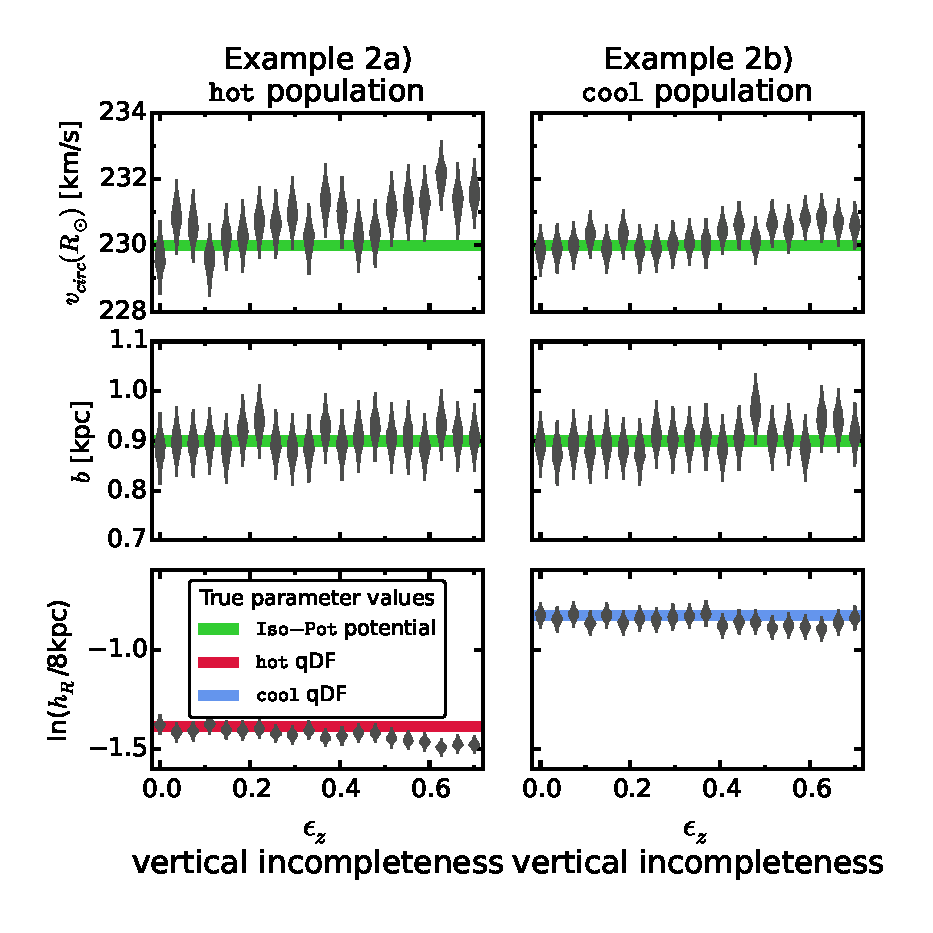
\includegraphics[width=0.8\textwidth]{figs/isoSphFlexIncompZ_violins_2.eps}
\caption{Influence of wrong assumptions about the incompleteness parallel to the Galactic plane of the data on the parameter reocovery with \RM{}. Each mock data set was created having different incompleteness parameters $\epsilon_z$ (shown on the $x$-axis and illustrated in Figure \ref{fig:isoSphFlexIncompZ_mockdata}) and the model parameters are given as Test \ref{test:isoSphFlexIncomp}, Example 2, in Table \ref{tbl:tests}. The analysis however didn't know about the incompleteness and assumed that all data sets had constant completeness within the survey volume ($\epsilon_z = 0$). The marginalized likelihoods from the fits are shown as violins. The green lines mark the true potential parameters (\texttt{Iso-Pot}) and the red and blue lines the true qDF parameters (\texttt{hot} \MAP{} in red and \texttt{cool} \MAP{} in blue), which we tried to recover. The \RM{} method seems to be robust against small to intermediate deviations between the true and the assumed vertical data incompleteness, as well as the radial incompleteness in Figure \ref{fig:isoSphFlexIncompZ_violins}.} 
\label{fig:isoSphFlexIncompZ_violins}
\end{minipage}
\end{figure}


\begin{figure*}
\plotone{figs/isoSphFlexIncomp_marginal_violins_2.eps}
\caption{Influence of wrong assumptions about radial and vertical incompleteness on the parameter recovery, when \emph{not} including information about the tangential velocities in the analysis. The mock data sets are the same as in Figure \ref{fig:isoSphFlexIncompR_violins} and \ref{fig:isoSphFlexIncompZ_violins}, but this time we did not include the data coordinates $v_T$ in the analysis and therefore marginalized the likelihood over $v_T$ instead (see \S\ref{sec:incompZ}). This demonstrates that much of the information about the potential is actually stored in the rotation curve, i.e. $v_T(R)$, which is not affected by removing stars from the data set. But even if we do not include $v_T$ we can still recover the potential within the errors, at least for small ($\epsilon_z \lesssim 10\%$).} 
\label{fig:isoSphFlexIncomp_marginal_violins}
\end{figure*}

\Wilma{[TO DO: Mention in text or caption how the panels looked that I removed.]}

%\end{appendix}







%
\begin{thebibliography}{}
\bibitem[Batsleer \& Dejonghe(1994)]{1994AA...287...43B} Batsleer, P., \& Dejonghe, H.\ 1994, \aap, 287, 43
\bibitem[Binney(2010)]{2010MNRAS.401.2318B} Binney, J.\ 2010, \mnras, 401, 2318
\bibitem[Binney \& McMillan(2011)]{2011MNRAS.413.1889B} Binney, J., \& McMillan, P.\ 2011, \mnras, 413, 1889
\bibitem[Binney(2011)]{2011Prama..77...39B} Binney, J.\ 2011, Pramana, 77, 39
\bibitem[Binney(2012)]{2012MNRAS.426.1324B} Binney, J.\ 2012, \mnras, 426, 1324
\bibitem[Binney(2012)]{2012MNRAS.426.1328B} Binney, J.\ 2012, \mnras, 426, 1328
\bibitem[Binney(2013)]{2013NewAR..57...29B} Binney, J.\ 2013, NAR \Wilma{[TO DO: emulateapj doesn't know NAR]}, 57, 29 
\bibitem[Binney \& Tremaine(2008)]{2008gady.book.....B} Binney, J., \& Tremaine, S.\ 2008, Galactic Dynamics: Second Edition, by James Binney and Scott Tremaine.~ISBN 978-0-691-13026-2 (HB).~Published by Princeton University Press, Princeton, NJ USA, 2008.
\bibitem[Bovy \& Tremaine(2012)]{2012ApJ...756...89B} Bovy, J., \& Tremaine, S.\ 2012, \apj, 756, 89
\bibitem[Bovy et al.(2012b)]{bov12b} Bovy, J., Rix, H.-W., \& Hogg, D. W. 2012b, \apj, 751, 131
\bibitem[Bovy et al.(2012c)]{bov12c} Bovy, J., Rix, H.-W., Hogg, D. W. et al., 2012c, \apj, 755,115
\bibitem[Bovy et al.(2012d)]{2012ApJ...753..148B} Bovy, J., Rix, H.-W., Liu, C., et al.\ 2012, \apj, 753, 148
\bibitem[Bovy \& Rix(2013)]{2013ApJ...779..115B} Bovy, J., \& Rix, H.-W.\ 2013, \apj, 779, 115
\bibitem[Bovy(2015)]{2015ApJS..216...29B} Bovy, J.\ 2015, \apjs, 216, 29 %[TO DO] bov15
\bibitem[B{\"u}denbender et al.(2015)]{2015MNRAS.452..956B} B{\"u}denbender, A., van de Ven, G., \& Watkins, L.~L.\ 2015, \mnras, 452, 956 
%\bibitem[Dehnen(1998)]{1998AJ....115.2384D} Dehnen, W.\ 1998, \aj, 115, 2384 
\bibitem[Dehnen \& Binney(1998)]{1998MNRAS.294..429D} Dehnen, W., \& Binney, J.\ 1998, \mnras, 294, 429 
\bibitem[de Lorenzi et al.(2007)]{2007MNRAS.376...71D} de Lorenzi, F., Debattista, V.~P., Gerhard, O., \& Sambhus, N.\ 2007, \mnras, 376, 71 
\bibitem[Famaey \& Dejonghe(2003)]{2003MNRAS.340..752F} Famaey, B., \& Dejonghe, H.\ 2003, \mnras, 340, 752 
\bibitem[Foreman-Mackey et al.(2013)]{2013PASP..125..306F} Foreman-Mackey, D., Hogg, D.~W., Lang, D., \& Goodman, J.\ 2013, \pasp, 125, 306
\bibitem[Garbari et al.(2012)]{2012MNRAS.425.1445G} Garbari, S., Liu, C., Read, J.~I., \& Lake, G.\ 2012, \mnras, 425, 1445 
\bibitem[Gilmore \& Reid(1983)]{1983MNRAS.202.1025G} Gilmore, G., \& Reid, N.\ 1983, \mnras, 202, 1025 
\bibitem[Henon(1959)]{1959AnAp...22..126H} Henon, M.\ 1959, Annales d'Astrophysique, 22, 126 
\bibitem[Holmberg et al.(2009)]{2009A&A...501..941H} Holmberg, J., Nordstr{\"o}m, B., \& Andersen, J.\ 2009, \aap, 501, 941 
\bibitem[Hunt \& Kawata(2014)]{hun14} Hunt, J. A. S., \& Kawata, D. 2014, \mnras, 443, 2112
\bibitem[Hunt \& Kawata(2014)]{2014MNRAS.443.2112H} Hunt, J.~A.~S., \& Kawata, D.\ 2014, \mnras, 443, 2112 
\bibitem[Juri{\'c} et al.(2008)]{2008ApJ...673..864J} Juri{\'c}, M., Ivezi{\'c}, {\v Z}., Brooks, A., et al.\ 2008, \apj, 673, 864 
\bibitem[Kawata et al.(2014)]{2014MNRAS.443.2757K} Kawata, D., Hunt, J.~A.~S., Grand, R.~J.~J., Pasetto, S., \& Cropper, M.\ 2014, \mnras, 443, 2757 
\bibitem[Klement et al.(2008)]{2008ApJ...685..261K} Klement, R., Fuchs, B., \& Rix, H.-W.\ 2008, \apj, 685, 261 
\bibitem[Kuijken \& Gilmore(1989)]{1989MNRAS.239..605K} Kuijken, K., \& Gilmore, G.\ 1989, \mnras, 239, 605 
\bibitem[McMillan(2011)]{2011MNRAS.414.2446M} McMillan, P.~J.\ 2011, \mnras, 414, 2446 %[TO DO] mcm11
\bibitem[McMillan(2012)]{2012EPJWC..1910002M} McMillan, P.~J.\ 2012, European Physical Journal Web of Conferences, 19, 10002 
\bibitem[McMillan \& Binney(2008)]{2008MNRAS.390..429M} McMillan, P.~J., \& Binney, J.~J.\ 2008, \mnras, 390, 429 
\bibitem[McMillan \& Binney(2012)]{2012MNRAS.419.2251M} McMillan, P.~J., \& Binney, J.\ 2012, \mnras, 419, 2251 
\bibitem[McMillan \& Binney(2013)]{2013MNRAS.433.1411M} McMillan, P.~J., \& Binney, J.~J.\ 2013, \mnras, 433, 1411 
%\bibitem[Navarro et al.(2004)]{2004ApJ...601L..43N} Navarro, J.~F., Helmi, A., \& Freeman, K.~C.\ 2004, \apjl, 601, L43 
%\bibitem[Ness et al.(2015)]{nes15} Ness, M., Hogg, D. W., Rix, H.-W. et al., 2015, \apj, 808, 16
\bibitem[Nordstr{\"o}m et al.(2004)]{2004A&A...418..989N} Nordstr{\"o}m, B., Mayor, M., Andersen, J., et al.\ 2004, \aap, 418, 989 
\bibitem[Perryman et al.(2001)]{2001A&A...369..339P} Perryman, M.~A.~C., de Boer, K.~S., Gilmore, G., et al.\ 2001, \aap, 369, 339 
\bibitem[Piffl et al.(2014)]{2014MNRAS.445.3133P} Piffl, T., Binney, J., McMillan, P.~J., et al.\ 2014, \mnras, 445, 3133
\bibitem[Read(2014)]{2014JPhG...41f3101R} Read, J.~I.\ 2014, Journal of Physics G Nuclear Physics, 41, 063101 
\bibitem[Rix \& Bovy(2013)]{2013A&ARv..21...61R} Rix, H.-W., \& Bovy, J.\ 2013, \aapr, 21, 61 %rix13 [TO DO]
%\bibitem[Sackett(1997)]{sac97} Sackett, P. 1997, \apj, 483, 103
\bibitem[Sanders \& Binney(2015)]{2015MNRAS.449.3479S} Sanders, J.~L., \& Binney, J.\ 2015, \mnras, 449, 3479
\bibitem[Sellwood(2010)]{2010MNRAS.409..145S} Sellwood, J.~A.\ 2010, \mnras, 409, 145 
\bibitem[Steinmetz et al.(2006)]{2006AJ....132.1645S} Steinmetz, M., Zwitter, T., Siebert, A., et al.\ 2006, \aj, 132, 1645 
\bibitem[Strigari(2013)]{2013PhR...531....1S} Strigari, L.~E.\ 2013, \physrep, 531, 1 
\bibitem[Syer \& Tremaine(1996)]{sye96} Syer D., Tremaine S. 1996, \mnras, 282, 223
\bibitem[Ting et al.(2013)]{2013MNRAS.434..652T} Ting, Y.-S., Rix, H.-W., Bovy, J., \& van de Ven, G.\ 2013, \mnras, 434, 652
\bibitem[Yanny et al.(2009)]{2009AJ....137.4377Y} Yanny, B., Rockosi, C., Newberg, H.~J., et al.\ 2009, \aj, 137, 4377 
\bibitem[Zhang et al.(2013)]{2013ApJ...772..108Z} Zhang, L., Rix, H.-W., van de Ven, G., et al.\ 2013, \apj, 772, 108
\end{thebibliography}
\HW{[TO DO: In which order should I give the references????]}
\\\Wilma{[TO DO: replace the references which I typed myself with the ones from ADS.]}
\\\Wilma{[TO DO: Check if all references are actually used in paper. ???]}
%-----------------------------------------------------------------------------------------------------------------------------------------------------------------------------
%Long landscape tables
\clearpage
\LongTables
\begin{landscape}
\begin{deluxetable}{lllll}%{p{0.1\textwidth}p{0.1\textwidth}p{0.25\textwidth}p{0.25\textwidth}p{0.05\textwidth}}
\tabletypesize{\scriptsize}
%\rotate
\tablecaption{Summary of test suites in this work: The first column indicates the test suite, the second column the potential, DF and selection function model etc. used for the mock data creation, the third model the corresponding model assumed in the analysis, and the last column lists the figures belonging to the test suite. Parameters that are not left free in the analyis, are always fixed to their true value. Unless otherwise stated we calculate the likelihood by the nested-grid and MCMC approach outlined in \S\ref{sec:fitting} and use $N_x = 16$, $N_v = 24$, $n_\sigma= 5$ as numerical accuracy for the likelihood normalisation in Equations (\ref{eq:prob}) and (\ref{eq:tracerdensity}). $N_{*}$ is the number of stars per mock data set. Unless stated otherwise, the all selection functions have completeness$(\vect{x}) = 1$. \Jo{[TO DO: Jo suggested to make many tables from this. But I actually like one big table at the end of the paper. Otherwise we had 6 additional tables interrupting the flow of text and figures all the time. And the parameters in the table are really just for reference.]} \Wilma{[TO DO: Overall, this table could do with a little less information.]} \label{tbl:tests}}
\tablewidth{0pt}
\tablehead{
\colhead{Test} & & \colhead{Model for Mock Data}  & \colhead{Model in Analysis} & \colhead{Figure}}
\startdata
Test \testlabel{test:kks2WedgeEx} {1}:        & \emph{Potential:}     & \texttt{KKS-Pot} & - & Figure \ref{fig:kks2WedgeEx}\\
Influence of            & \emph{DF:}          & \texttt{hot} or \texttt{cool} qDF   &   & \\
survey volume on        & \emph{Survey volume:} & a) $R \in [4,12]$ kpc,$z \in [-4,4]$ kpc, $\phi \in [-20^\circ,20^\circ]$. &  & \\
mock data distribution, &                       & b) $R \in [6,10]$ kpc,$z \in [1,5]$ kpc, $\phi \in [-20^\circ,20^\circ]$.&  & \\
also in action space	& \emph{$N_{*}$:} & 20,000 &  & \\

\tableline
Test \testlabel{test:norm_accuracy} {2}:         & \emph{Potential:}     & \texttt{KKS-Pot} & - & Figure \ref{fig:norm_accuracy}\\
Numerical accuracy      & \emph{DF:}          & \texttt{hot} qDF                          &   & \\
in calculation          & \emph{Survey volume:} & sphere around Sun, $r_\text{max} = 0.2, 1, 2, 3$ or $4$ kpc &   & \\
of the likelihood       & \emph{Numerical accuracy:} & $N_x\in[5,20]$, $N_v\in[6,40]$, $n_\sigma\in[3.5,7]$& & \\
normalisation           &                       & & & \\
										   
\tableline
Test \testlabel{test:isoSphFlex} {3.1}:      & \emph{Potential:}     & \texttt{Iso-Pot} & \texttt{Iso-Pot}, all parameters free & Figure \ref{fig:isoSphFlex_triangleplot}\\
\pdf{} is a               & \emph{DF:}          & \texttt{hot} qDF & qDF, all parameters free & \\
multivariate            & \emph{Survey Volume:} & sphere around Sun, $r_\text{max} = 2$ kpc & (fixed \& known) & \\
Gaussian                & \emph{$N_{*}$:} & 20,000 & & \\
for large data sets.	&  \emph{Numerical accuracy:} & & $N_v = 20$ and $n_\sigma = 4$ & \\

\tableline
Test \testlabel{test:sqrtNiso} {3.2}:			& \emph{Potential:}     & \texttt{Iso-Pot} & \texttt{Iso-Pot}, free parameter: $b$ & Figure \ref{fig:sqrtNiso}\\
Width of the			& \emph{DF:}          & \texttt{hot} qDF & \texttt{hot} qDF, free parameters: & \\
likelihood scales       &                       &           & $\ln h_R,\ln\sigma_{R,0},\ln h_{\sigma,R}$ & \\
with number of stars    & \emph{Survey volume:} & sphere around Sun, $r_\text{max} = 3$ kpc   & (fixed \& known) & \\
by $\propto 1/\sqrt{N_{*}}$.& \emph{$N_{*}$:} & between 100 and 40,000 &  & \\                              
                        & \emph{Analysis method:} & & likelihood on grid & \\
                        & \emph{Numerical accuracy:} & & $N_v = 20$ and $n_\sigma = 4$ (for speed) & \\

\tableline
Test \testlabel{test:isoSph_CLT} {3.3}:        & \emph{Potential:}     & \texttt{Iso-Pot} & \texttt{Iso-Pot}, free parameter: $b$ & Figure \ref{fig:isoSph_CLT}\\
Parameter estimates     & \emph{DF:}       &\texttt{hot} or \texttt{cool} qDF & \texttt{hot}/\texttt{cool} qDF, free parameters:\\
are unbiased.           &          &    & $\ln h_R,\ln\sigma_{R,0},\ln h_{\sigma,R}$ & \\
                        & \emph{Survey volume:} & 5 spheres around Sun, $r_\text{max} = 0.2, 1, 2, 3$ or $4$ kpc & (fixed \& known) & \\
                        & \emph{$N_{*}$:} & 20,000 & & \\
                        & \emph{Analysis method:} & & likelihood on grid & \\
                        & \emph{Numerical accuracy:} & & $N_v = 20$ and $N_\sigma = 4$ (for speed) & \\

\tableline
Test \testlabel{test:wedFlexVol} {4} :		& \emph{Potential:} 	& i) \texttt{Iso-Pot} or ii) \texttt{MW13-Pot} & i) \texttt{Iso-Pot}, all parameters free & Figure \ref{fig:wedFlexVol_bias_vs_SE} \\
Influence of 			& 						& 													& ii) \texttt{MW13-Pot}, $R_d$ and $f_h$ free & \\
position \& shape 		& \emph{DF:}			& \texttt{hot} qDF 										& i) qDF, all parameters free & \\
of survey volume 		& 						& 													& ii) qDF, only $h_R$, $\sigma_{z,0}$ and $h_{\sigma,R}$ free& \\
on parameter recovery 	& \emph{Survey volume:}	& 4 different wedges, see Figure \ref{fig:wedFlexVol_bias_vs_SE}, upper right panel & (fixed \& known) & \\
						& \emph{$N_{*}$:} & 20,000 & & \\
						& \emph{Analysis method:} & & i) MCMC, ii) likelihood on grid & \\
\tableline
Test \testlabel{test:isoSphFlexIncomp}{5} :        & \emph{Potential:}     & \texttt{Iso-Pot} & \texttt{Iso-Pot}, all parameters free & Figure \ref{fig:isoSphFlexIncompR_violins} \& \ref{fig:isoSphFlexIncompR_marginal_violins}\\
Influence of            & \emph{DF:}          & \texttt{hot} or \texttt{cool} qDF & qDF, all parameters free &   \\
wrong assumptions       & \emph{Survey volume:} & sphere around Sun, $r_\text{max} = 3$ kpc & (fixed \& known) & \\
about the data set      & \emph{Completeness:}  & radial incompleteness (see Figure \ref{fig:isoSphFlexIncompR_completeness_shapes}),  & data set complete, & \\
(in-)completeness       &                       & completeness$(r) = 1-\epsilon_r \frac{r}{r_\text{max}}$, $\epsilon_r \in [0,0.7]$ & completeness$(r)$ = 1, $\epsilon_r=0$& \\
on parameter recovery   &                       & $r \equiv$ distance from Sun, & & \\
                        & \emph{$N_{*}$:} & 20,000 & & \\
\tableline
Test \testlabel{test:isoSphFlexErrConv_MC_vs_error}{6.1} :		& \emph{Potential:} 	& \texttt{Iso-Pot} & \texttt{Iso-Pot}, all parameters free" & Figure \ref{fig:isoSphFlexErrConv_MC_vs_error}\\
Numerical convergence 	& \emph{DF:}			& \texttt{hot} qDF & qDF, all parameters free & \\
of convolution		& \emph{Survey Volume:}	& sphere around Sun, $r_\text{max} = 3$ kpc & (fixed \& known) & \\
with measurement		& \emph{Uncertainties:}		& $\delta \text{RA} =\delta \text{DEC} =\delta(m-M)=0$	& (fixed \& known)	& \\
uncertainties					&						& $\delta v_\text{los} = 2$ km/s	&  & \\
						&						& $\delta \mu_\text{RA}= \delta \mu_\text{DEC}  =$ 2,3,4 or 5 mas/yr & & \\
						& \emph{Numerical Accuracy:} & & $N_\text{error} \in [25,1200]$& \\
						& \emph{$N_{*}$:} & 10,000 & & \\
\tableline
Test \testlabel{test:isoSphFlexErrConv_SE_vs_error}{6.2} : & \emph{Potential:} & \texttt{Iso-Pot} & \texttt{Iso-Pot}, all parameters free & Figure \ref{fig:isoSphFlexErrConv_SE_vs_error}\\
Effect of proper motion & \emph{DF:} & \texttt{hot} or \texttt{cool} qDF & qDF, all parameters free & \\
uncertainties on & \emph{Survey volume:} & sphere around Sun, $r_\text{max} = 3~\text{kpc}$ & (fixed \& known) & \\
precision of & \emph{Uncertainties:} & a) $\delta\text{RA}=\delta\text{DEC}=\delta(m-M)=0,$ & (fixed \& known) & \\
potential recovery & & $\delta v_\text{los} = 2~\text{km s}^{-1},$ & & \\
& & $\delta \mu_\text{RA}=\delta \mu_\text{DEC}=$ 1,2,3,4 or 5 $\text{mas yr}^{-1}$ & & \\
& & b) no measurement uncertainties & & \\
 & \emph{$N_{*}$:} & 10,000 & & \\
\tableline
Test \testlabel{test:isoSphFlexErrConv_bias_vs_SE}{6.3} : & \emph{Potential:} 	& \texttt{Iso-Pot} & \texttt{Iso-Pot}, all parameters free & Figure \ref{fig:isoSphFlexErrConv_bias_vs_SE}\\
Testing the	convolution		& \emph{DF:}			& \texttt{hot} qDF & qDF, all parameters free & \\
with measurement 		& \emph{Survey Volume:}	& sphere around Sun, $r_\text{max} = 3$ kpc & (fixed \& known) & \\
 uncertainties  & \emph{Uncertainties:}		& $\delta \text{RA} =\delta \text{DEC} =0$,	& fixed \& known,	& \\
with \& without			&						& $\delta v_\text{los}  = 2~\text{km s}^{-1}$, & but treatment of distance & \\
distance uncertainties						&						& $\delta \mu_\text{RA} = \delta \mu_\text{DEC} =$ 1,2,3,4 or 5 $\text{mas yr}^{-1}$, & uncertainties following & \\
						&						& a) $\delta(m-M) = 0$  or & Section \ref{sec:likelihood}&  \\
						&                     & b) $\delta(m-M) \neq 0$.  & & \\
						&                     &  (see Figure \ref{fig:isoSphFlexErrConv_bias_vs_SE})  & & \\
						& \emph{$N_{*}$:} & 10,000 & & \\
\tableline
Test \testlabel{test:isoSphFlexErrSyst}{6.4} :	& \emph{Potential:}		& \texttt{Iso-Pot} & \texttt{Iso-Pot}, all parameters free & Figure \ref{fig:isoSphFlexErrSyst}\\
Underestimation 	& \emph{DF:}			& \texttt{hot} or \texttt{cool} qDF & qDF, all parameters free & \\
of proper motion 	& \emph{Survey volume:}	& sphere around Sun, $r_\text{max} = 3$ kpc & (fixed \& known) & \\
uncertainties 			 	& \emph{Uncertainties:}		& only proper motion errors & proper motion uncertainties & \\
					&						& 1, 2 or 3 mas/yr & 10\% or 50\% underestimated & \\
					& \emph{$N_{*}$:} & 10,000 & & \\
\tableline
Test \testlabel{test:isoSphFlexMix}{7} :       & \emph{Potential:} & \texttt{Iso-Pot} & \texttt{Iso-Pot}, all parameters free & Figures \ref{fig:isoSphFlexMixCont} \& \ref{fig:isoSphFlexMixDiff}\\
Deviations in the       & \emph{DF:}      & mix of two qDFs (see Figure \ref{fig:isoSphFlexMix_mockdata_residuals})& single qDF, all parameters free & \\
assumed DF              &                   & \emph{Example 1:}   & & \\
from the                &                   & fixed qDF parameters & & \\
star's true DF          &                   & (\texttt{hot} \& \texttt{cooler} qDF from Table \ref{tbl:referenceMAPs}) & & \\
                        &                   & but different mixing rates. & & \\
                        &                   & \emph{Example 2:} & & \\
                        &                   & 50/50 mixture & & \\
                        &                   & with varying qDF parameters (by $X\%$): & & \\
                        &                   & a) \texttt{hot} \& \texttt{colder} qDF or & & \\
                        &					  & b) \texttt{cool} \& \texttt{warmer} qDF (see Table \ref{tbl:referenceMAPs}) & & \\
                        & \emph{Survey volume:}& sphere around Sun, $r_\text{max}=2$ kpc & (fixed \& known) & \\
                        & \emph{$N_{*}$:} & 20,000 & & \\
                        \tableline
Test \testlabel{test:MW14vsKKS2SphFlex}{8} :			&  \emph{Potential:} & \texttt{MW14-Pot} & \texttt{KKS-Pot}, all parameters free, & potential contours: \\
Deviations of the		&                    &            & only $v_\text{circ}(R_\odot)=230 \text{km s}^{-1}$ fixed & Figure \ref{fig:MW14vsKKS2SphFlex} \\
assumed potential model	& \emph{DF:}       & \texttt{hot} or \texttt{cool} qDF & qDF, all parameters free & qDF recovery: \\
from the star's			& \emph{Survey volume:} & sphere around Sun, $r_\text{max} = 4$ kpc & (fixed \& known) & Figure \ref{fig:MW14vsKKS2SphFlex_violins}\\
true potential			& \emph{$N_{*}$:} & 20,000 & & \\
\enddata
\end{deluxetable}



\clearpage
\end{landscape}


%-----------------------------------------------------------------------------------------------------------------------------------------------------------------------------

\end{document}

